\section{User Interface Representation (Of  Respective Project)}

The applications interface is designed using custom art elements, the functionality is implemented using Android SDK, and the phase of testing the product was accomplished successfully. The application can very well manage,store and share different E-books among different users. User can upload and download E-books based upon preference.User can also enter
Description, date , name  and other optional attributes ( Adding categories  to the E-books). With this entered information, the user is able to see the name, file size, description, upload date and many other details of ebook.


\subsection{Snapshots of system }


\begin{figure}[ht]
\centering
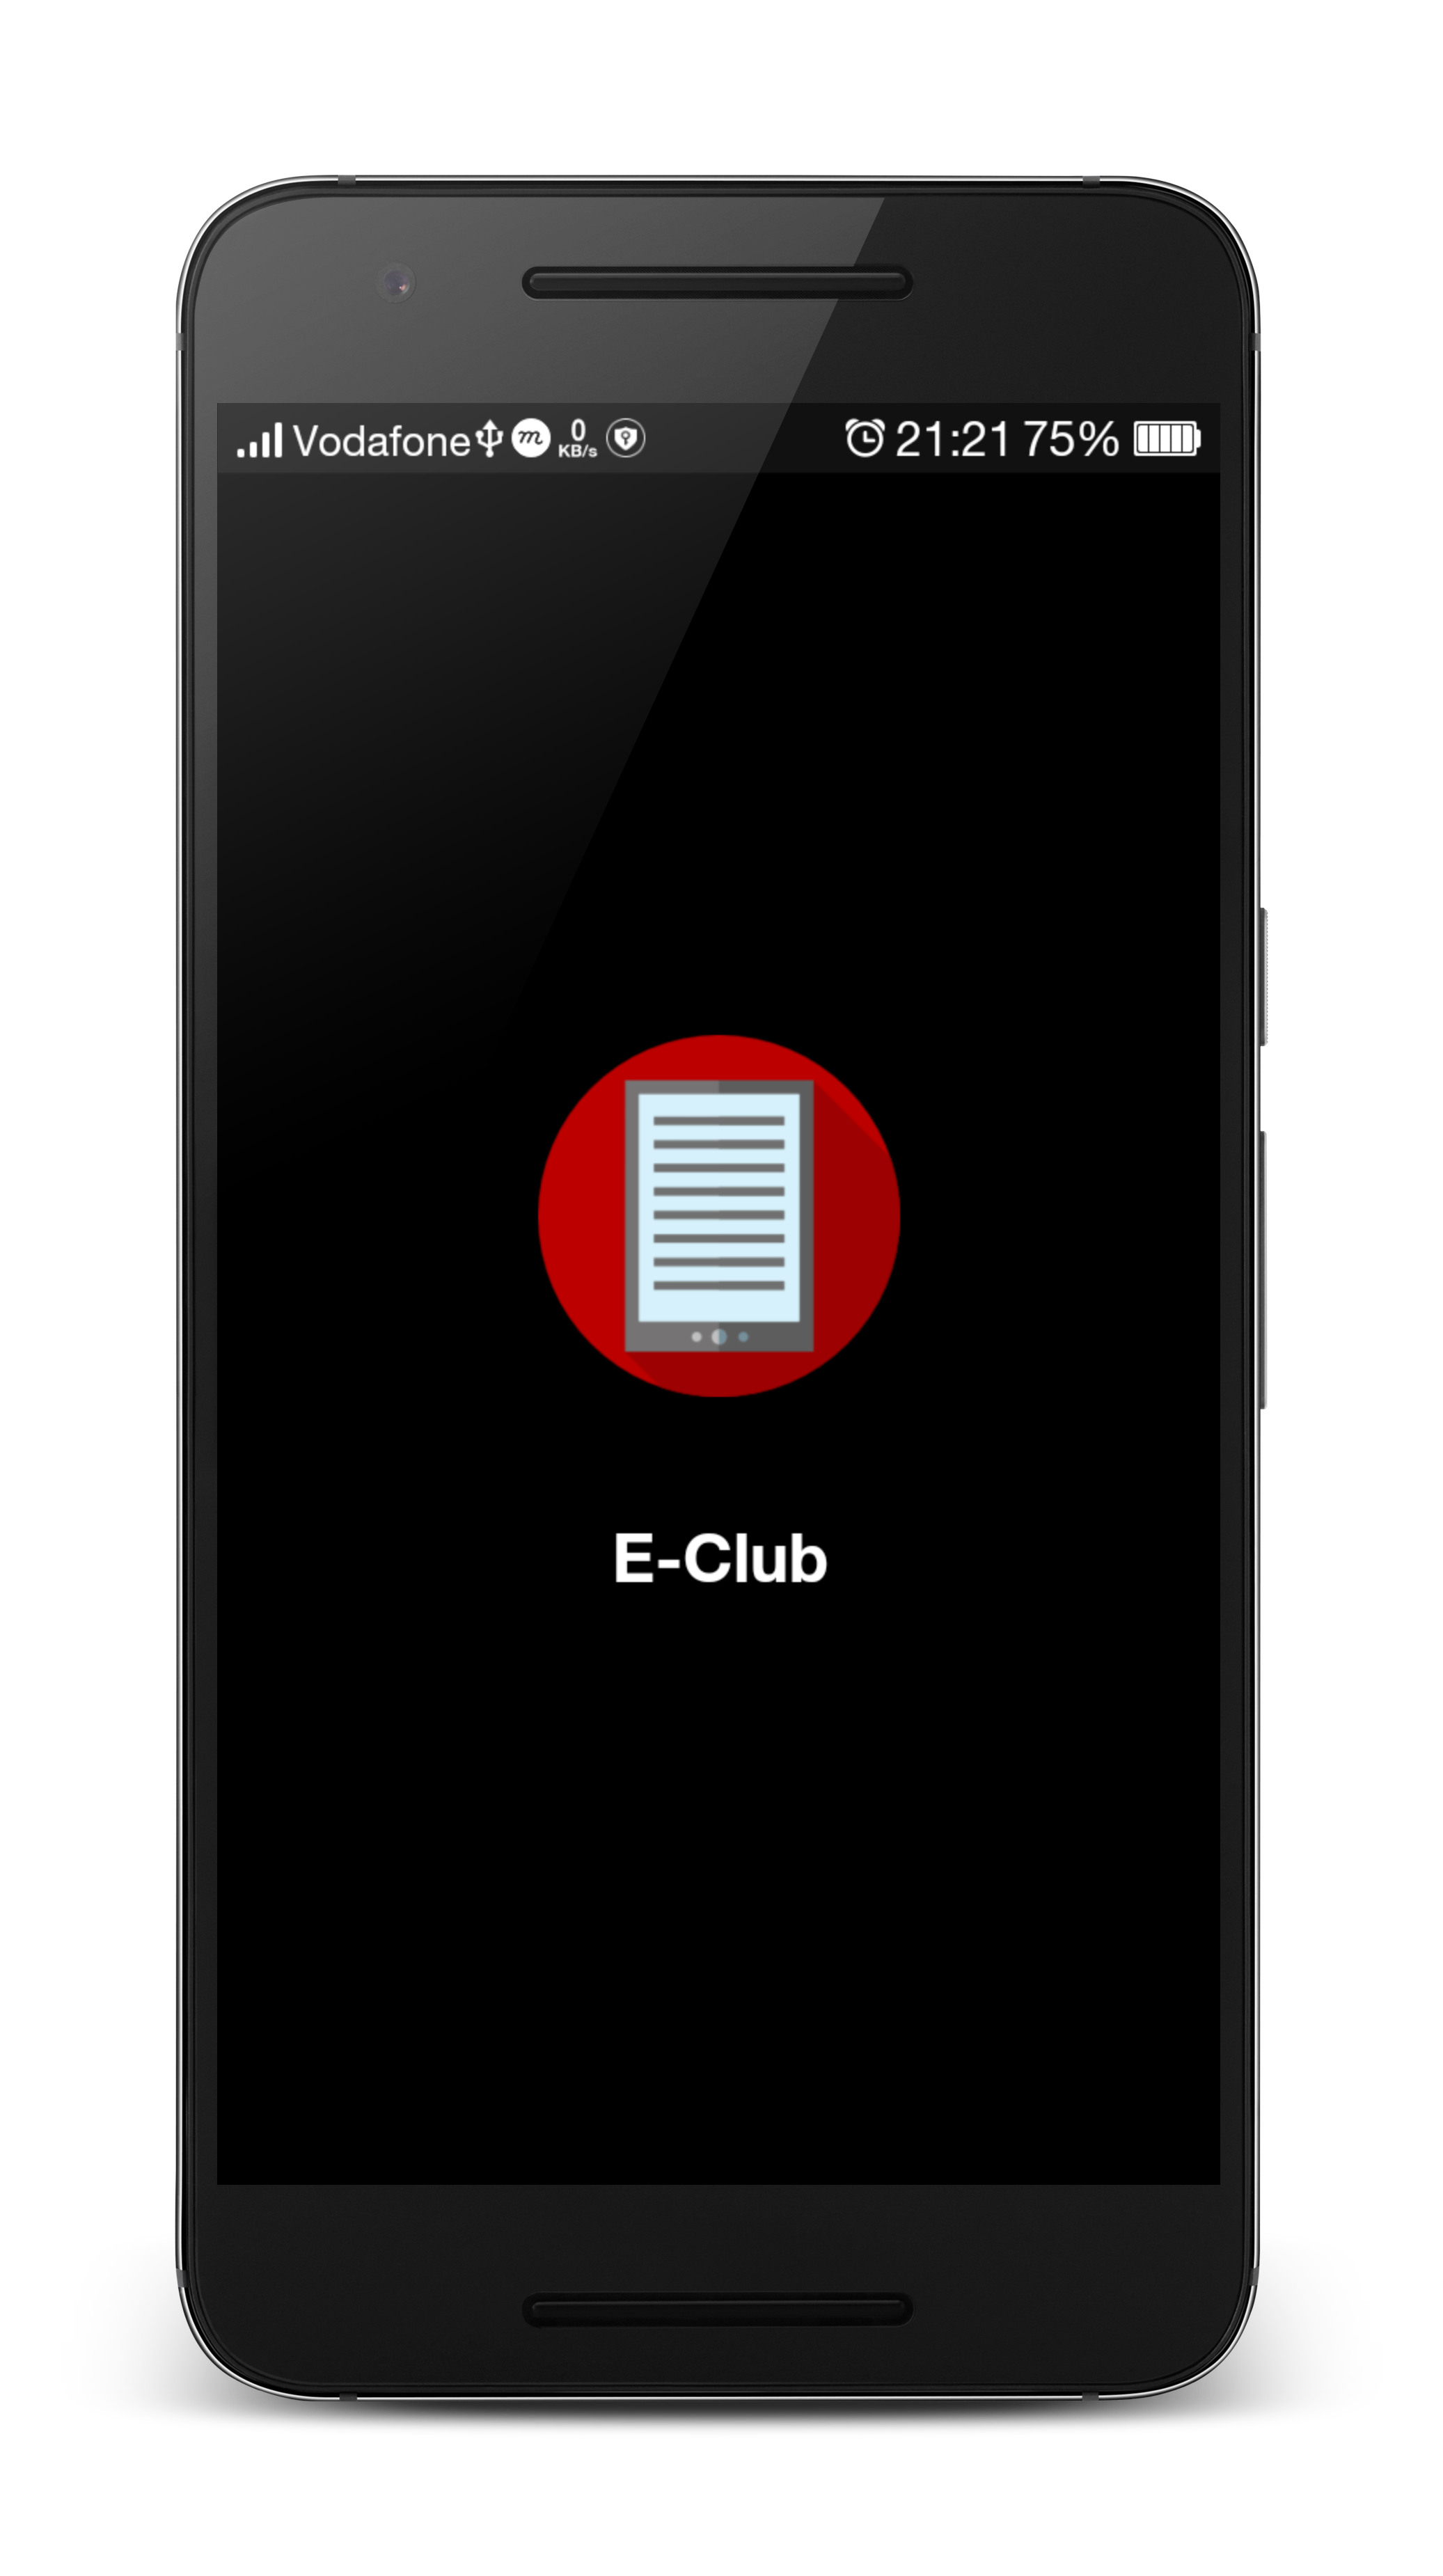
\includegraphics[scale=0.06]{images/d16.png}
\caption{Screen 1}
\end{figure}

\newpage

\begin{figure}[ht]
\centering
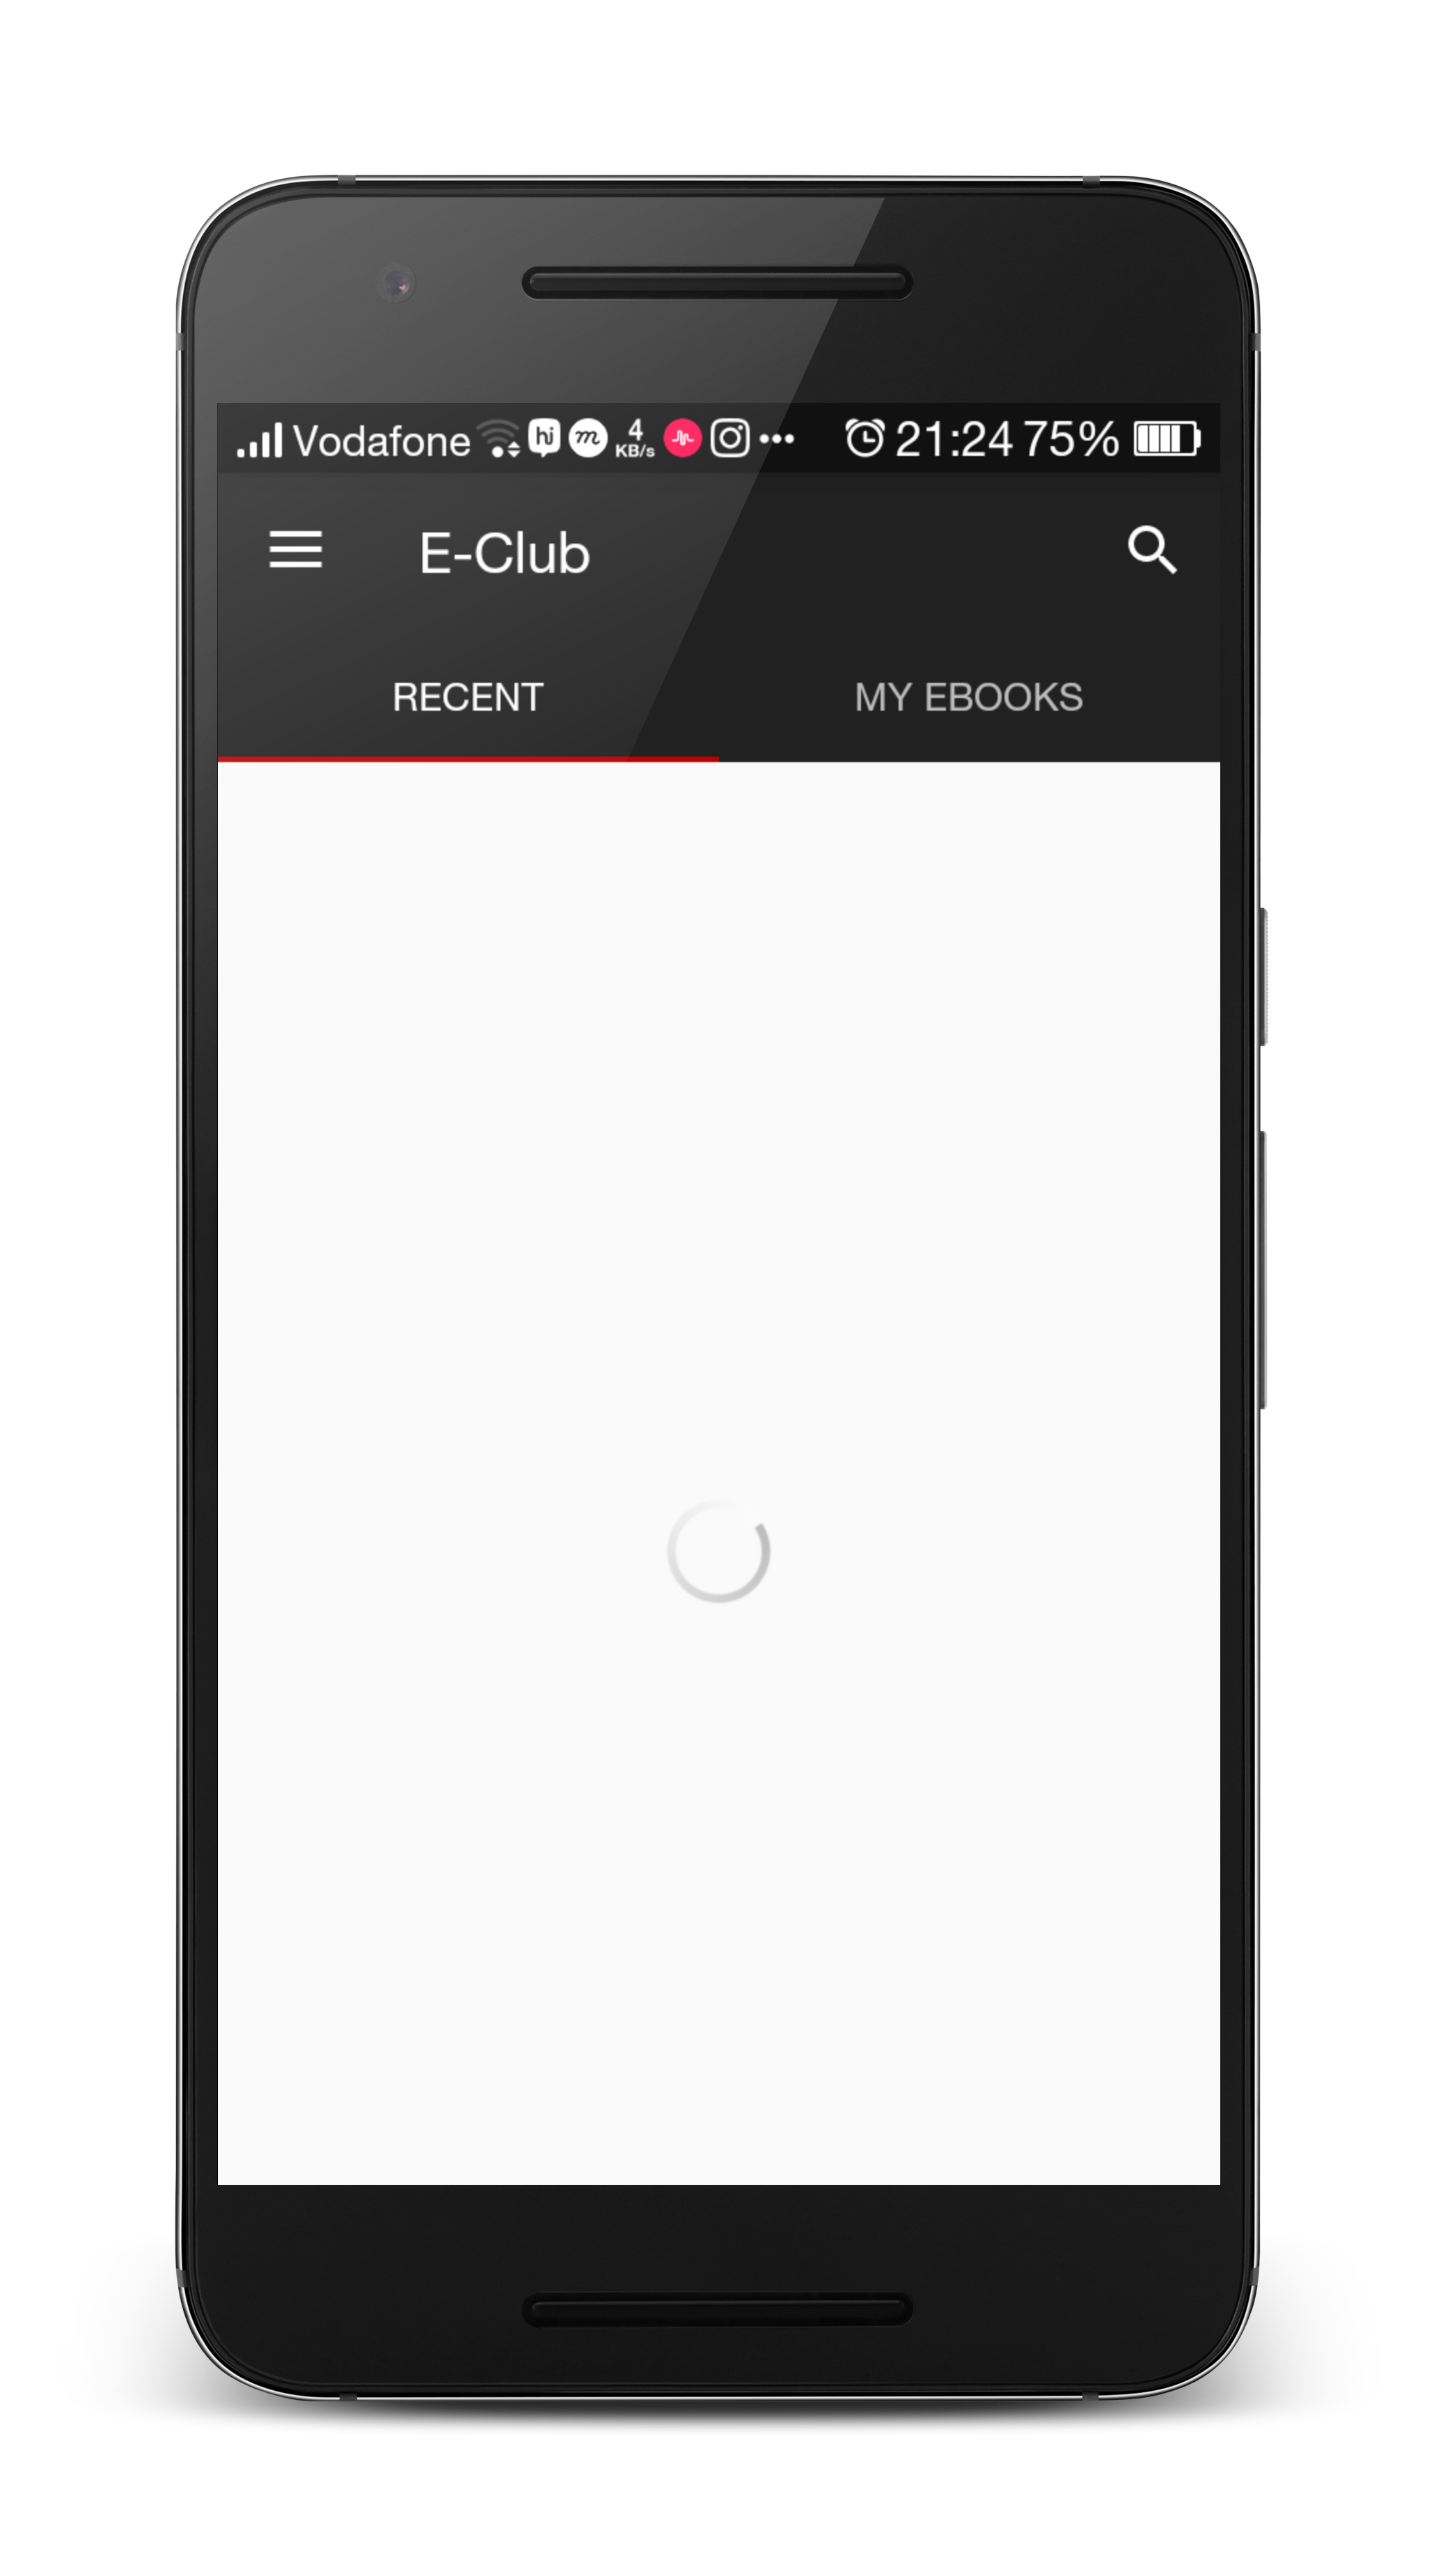
\includegraphics[scale=0.13]{images/d15.png}
\caption{Screen 2}
\end{figure}

\newpage


\begin{figure}[ht]
\centering
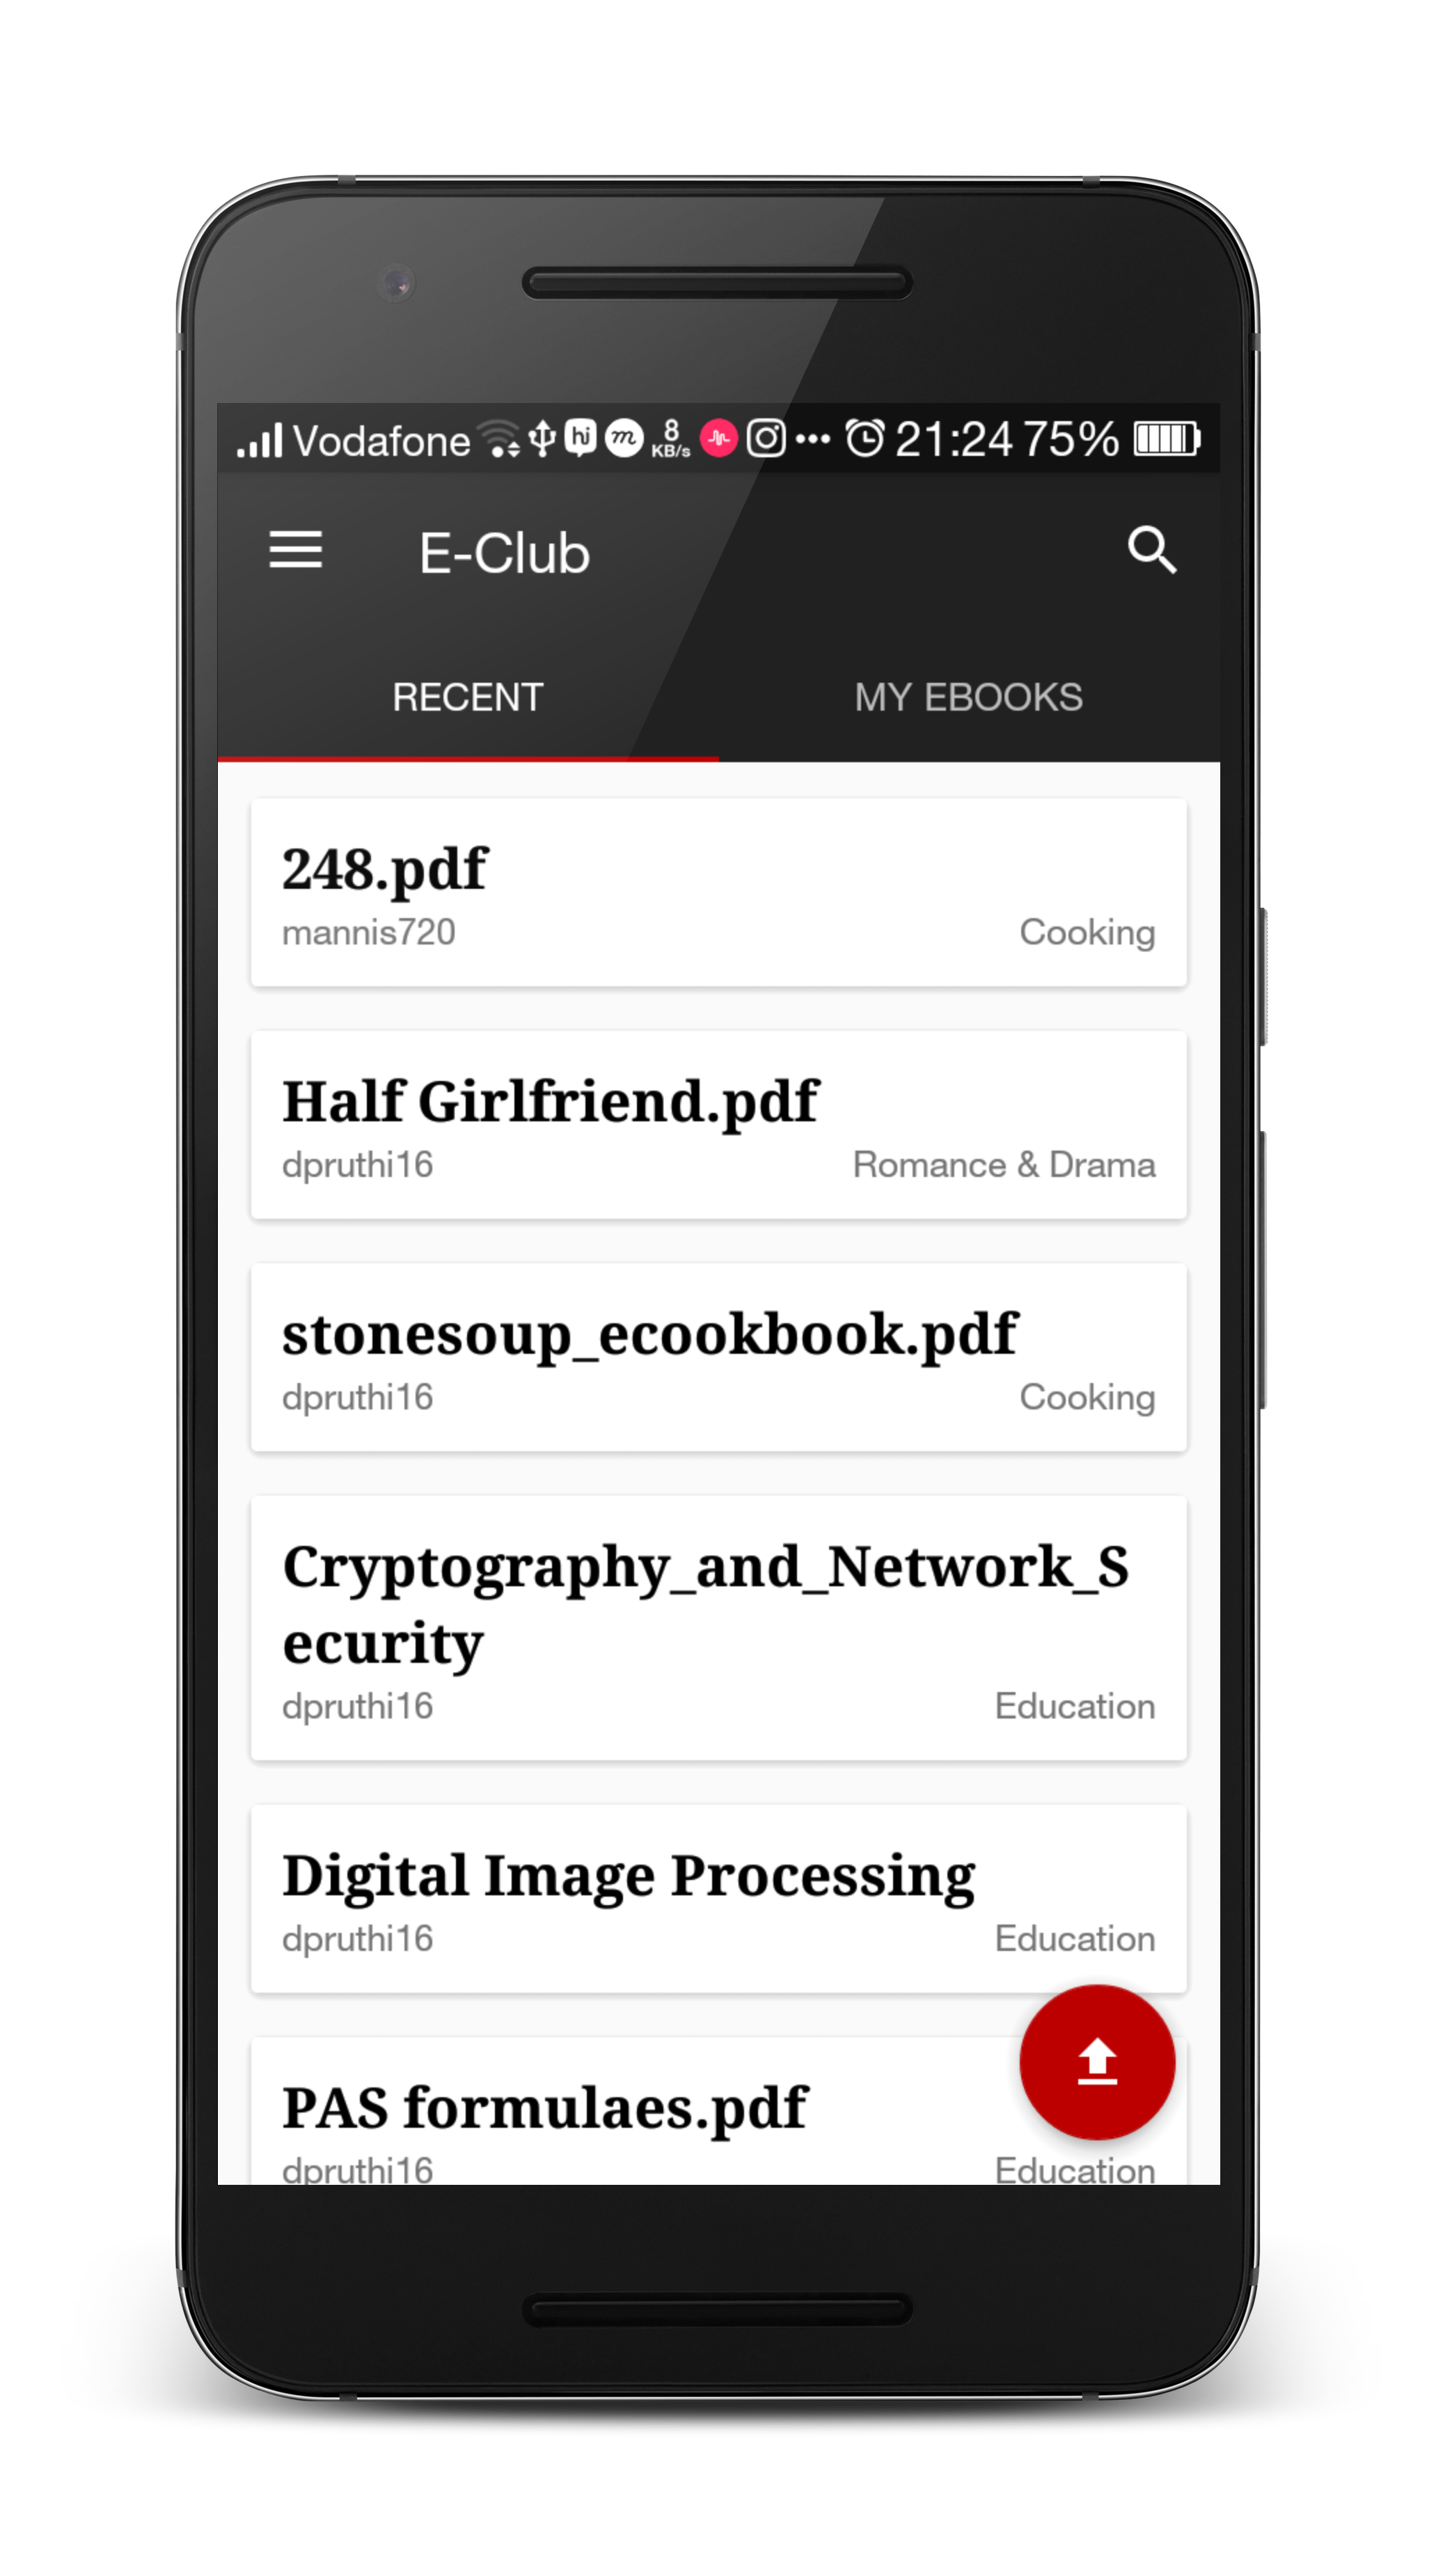
\includegraphics[scale=0.13]{images/d14.png}
\caption{Screen 3}
\end{figure}

\newpage

\begin{figure}[ht]
\centering
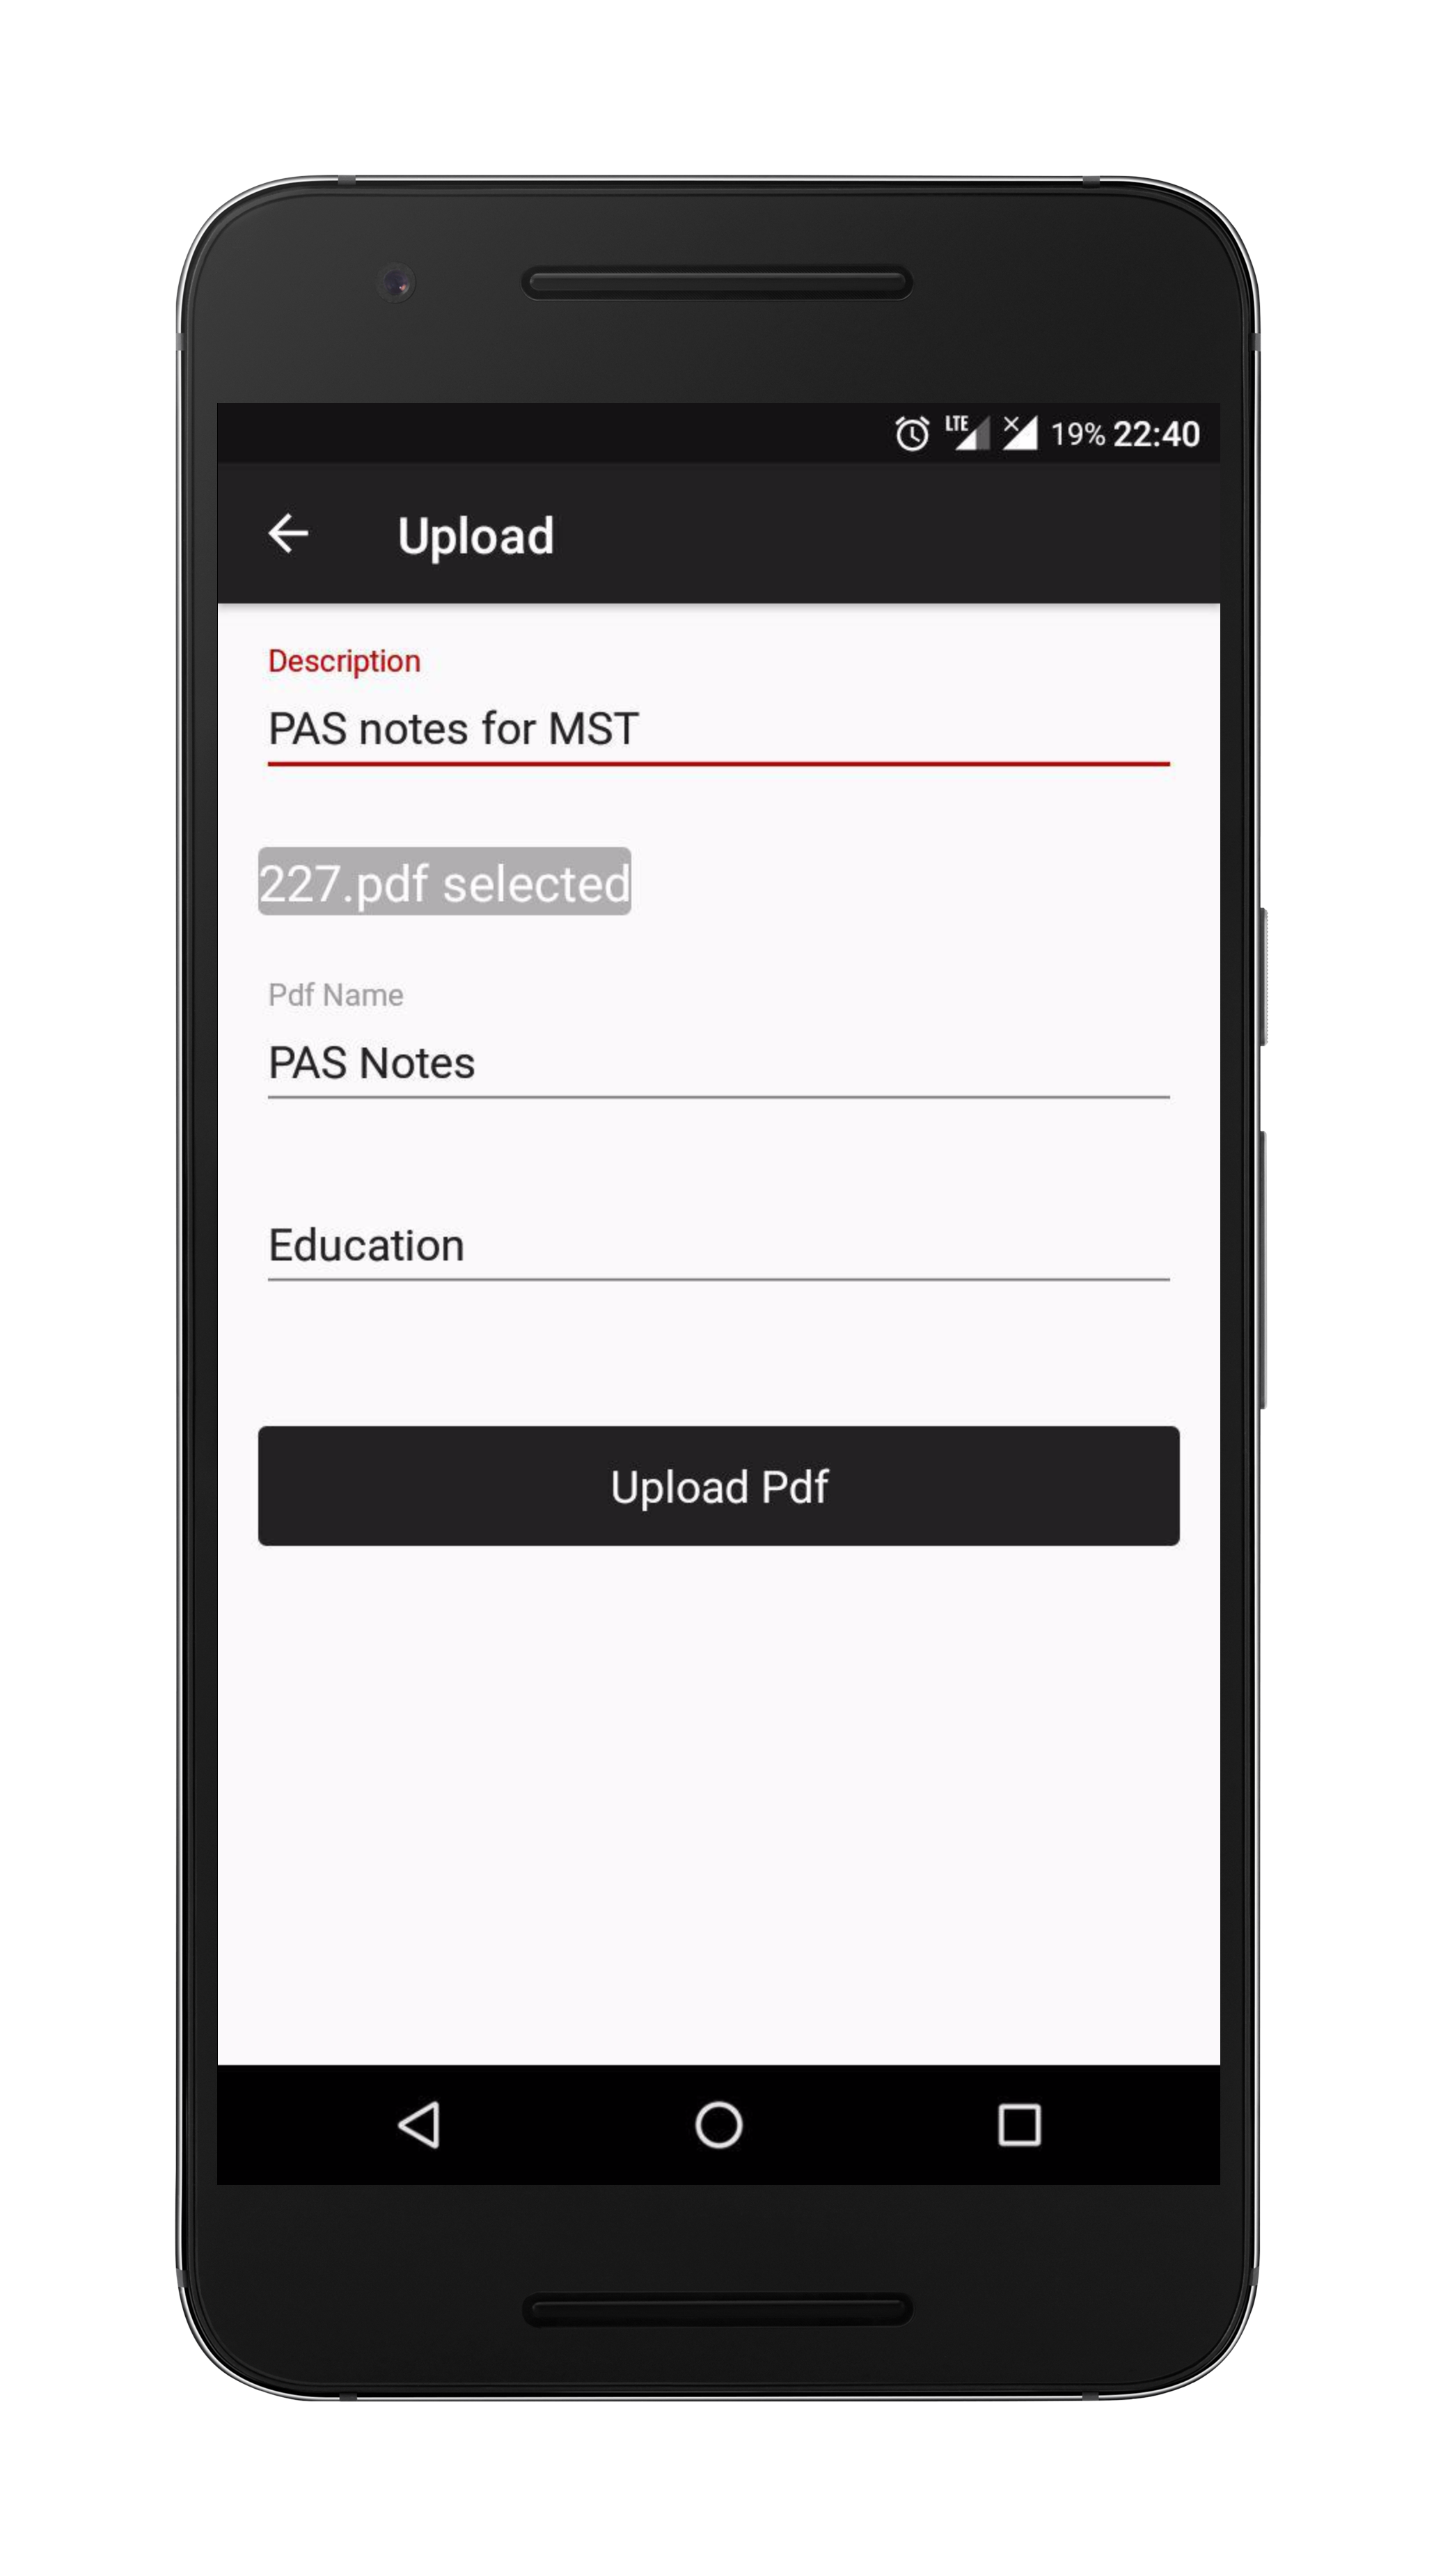
\includegraphics[scale=0.13]{images/up.png}
\caption{Screen 4}
\end{figure}

\newpage

\begin{figure}[ht]
\centering
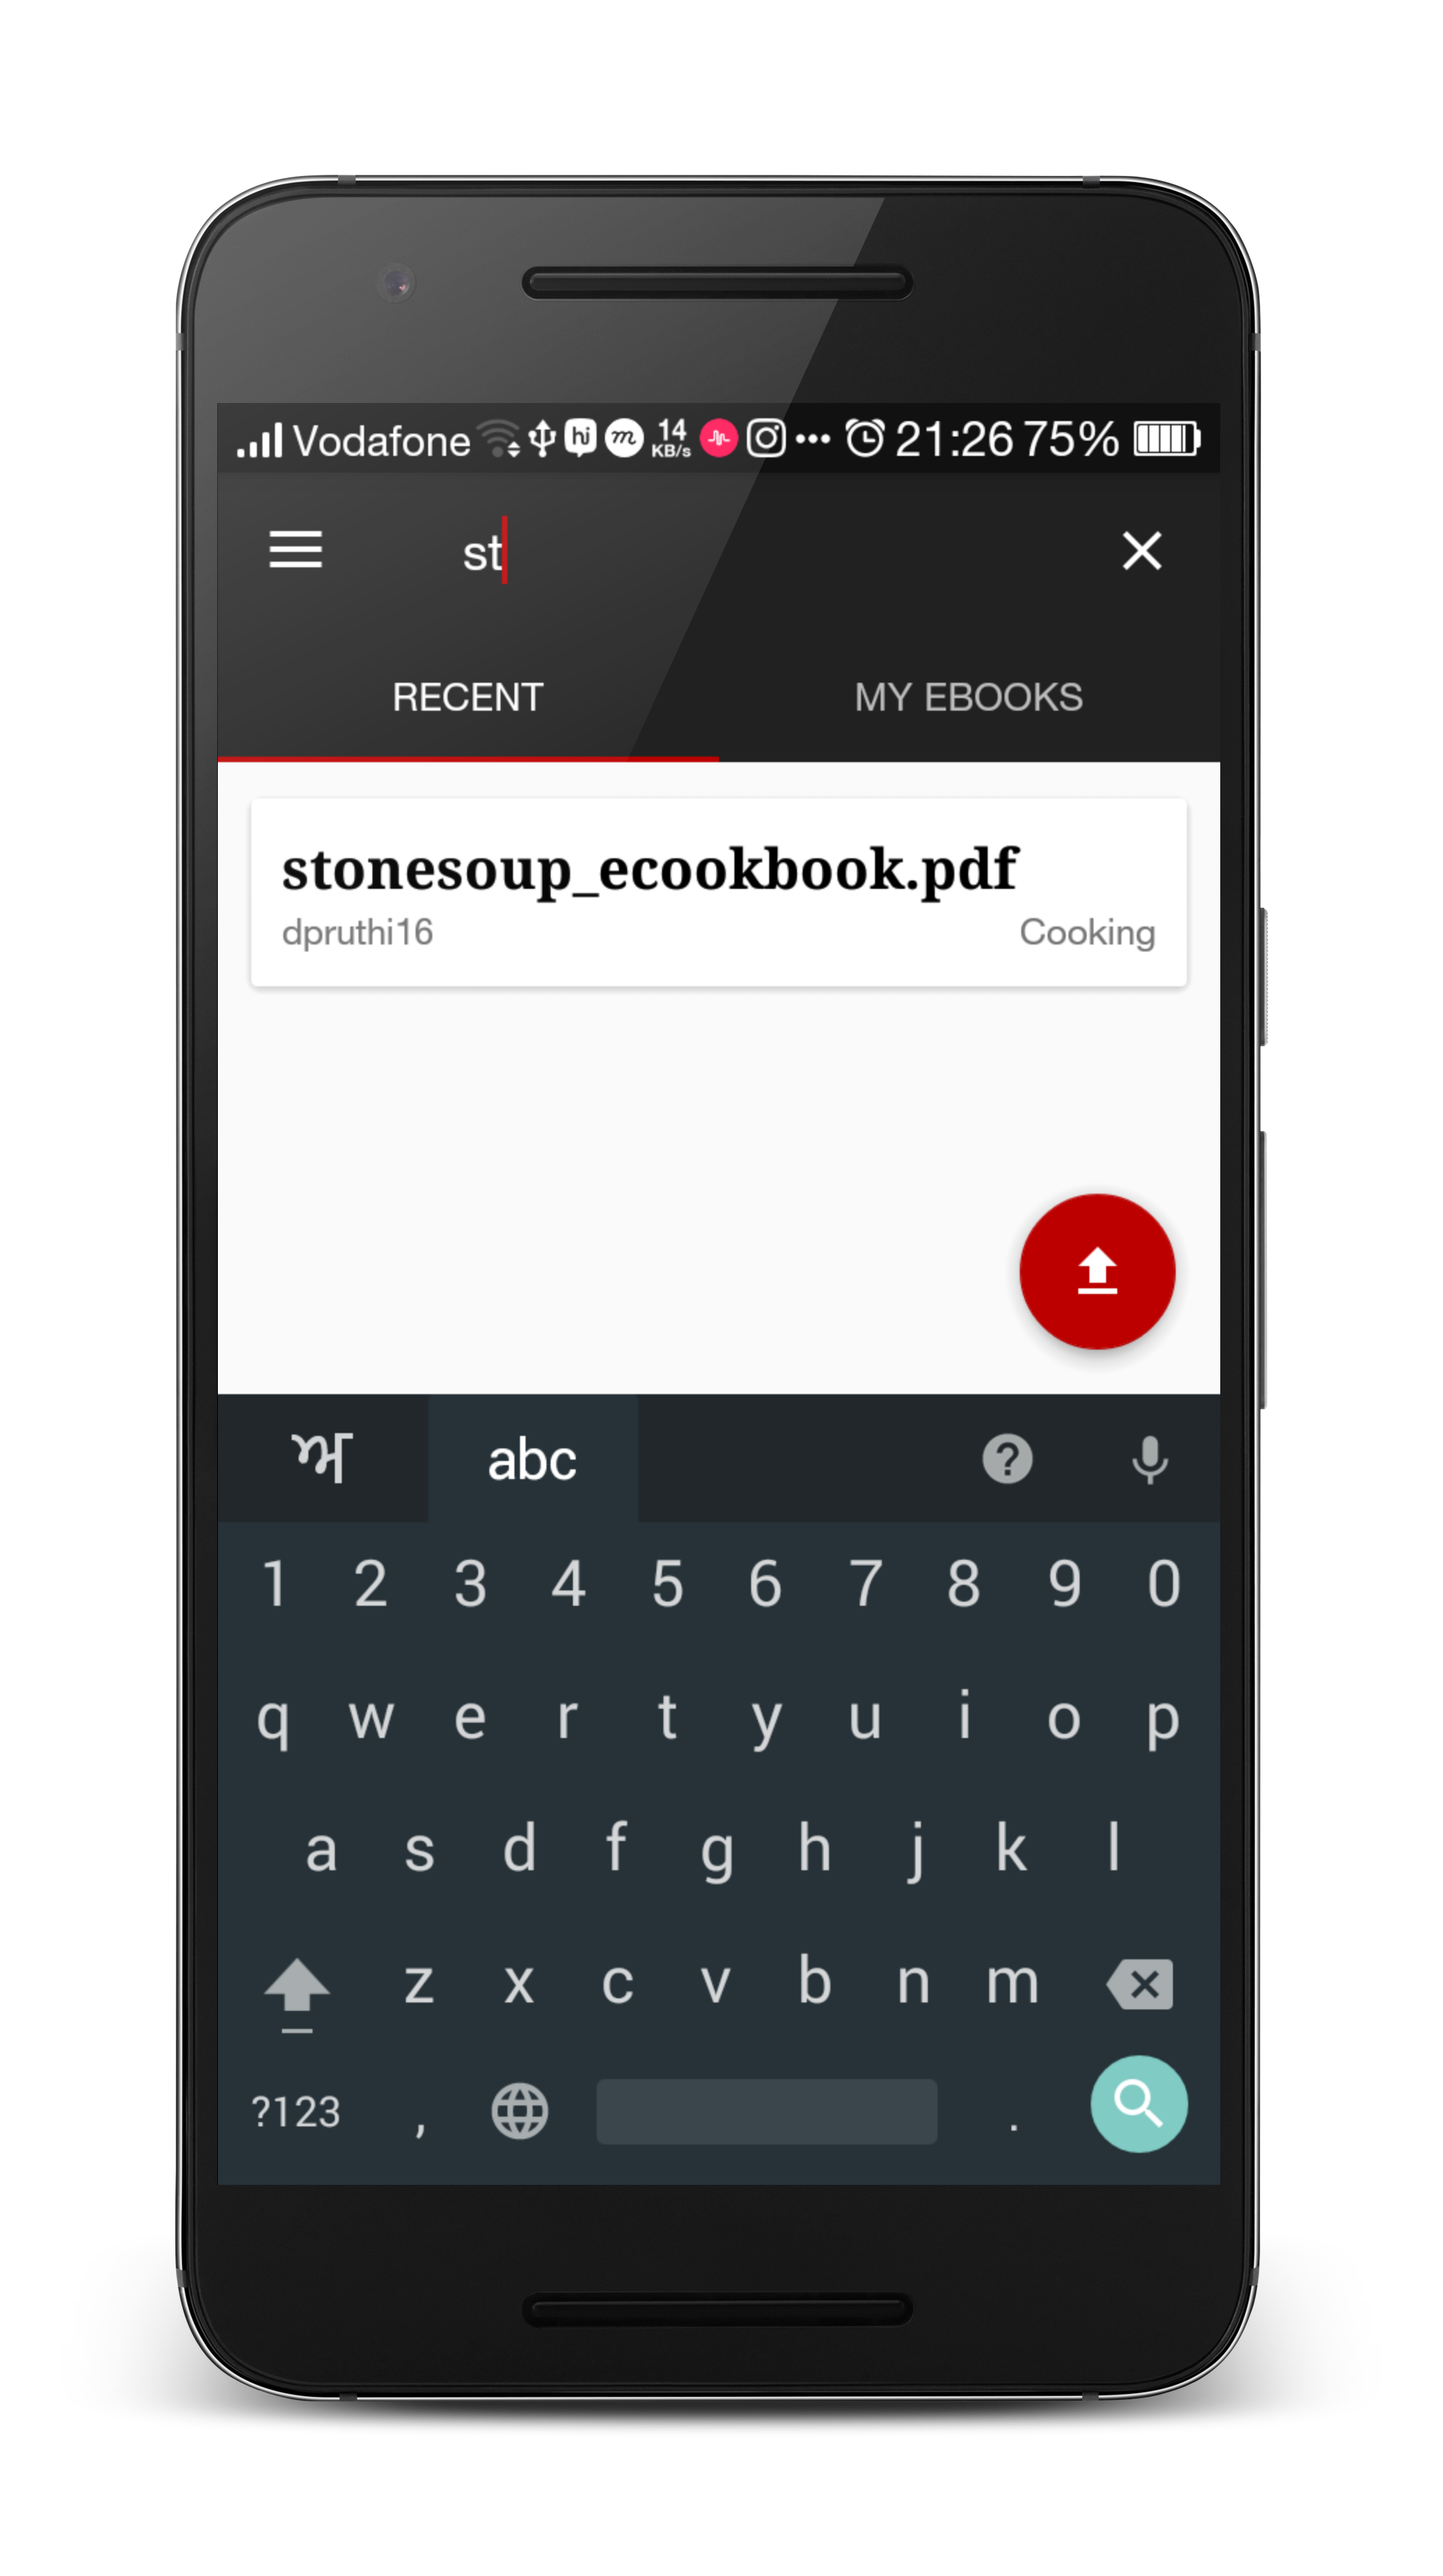
\includegraphics[scale=0.13]{images/d10.png}
\caption{Screen 5}
\end{figure}

\newpage

\begin{figure}[ht]
\centering
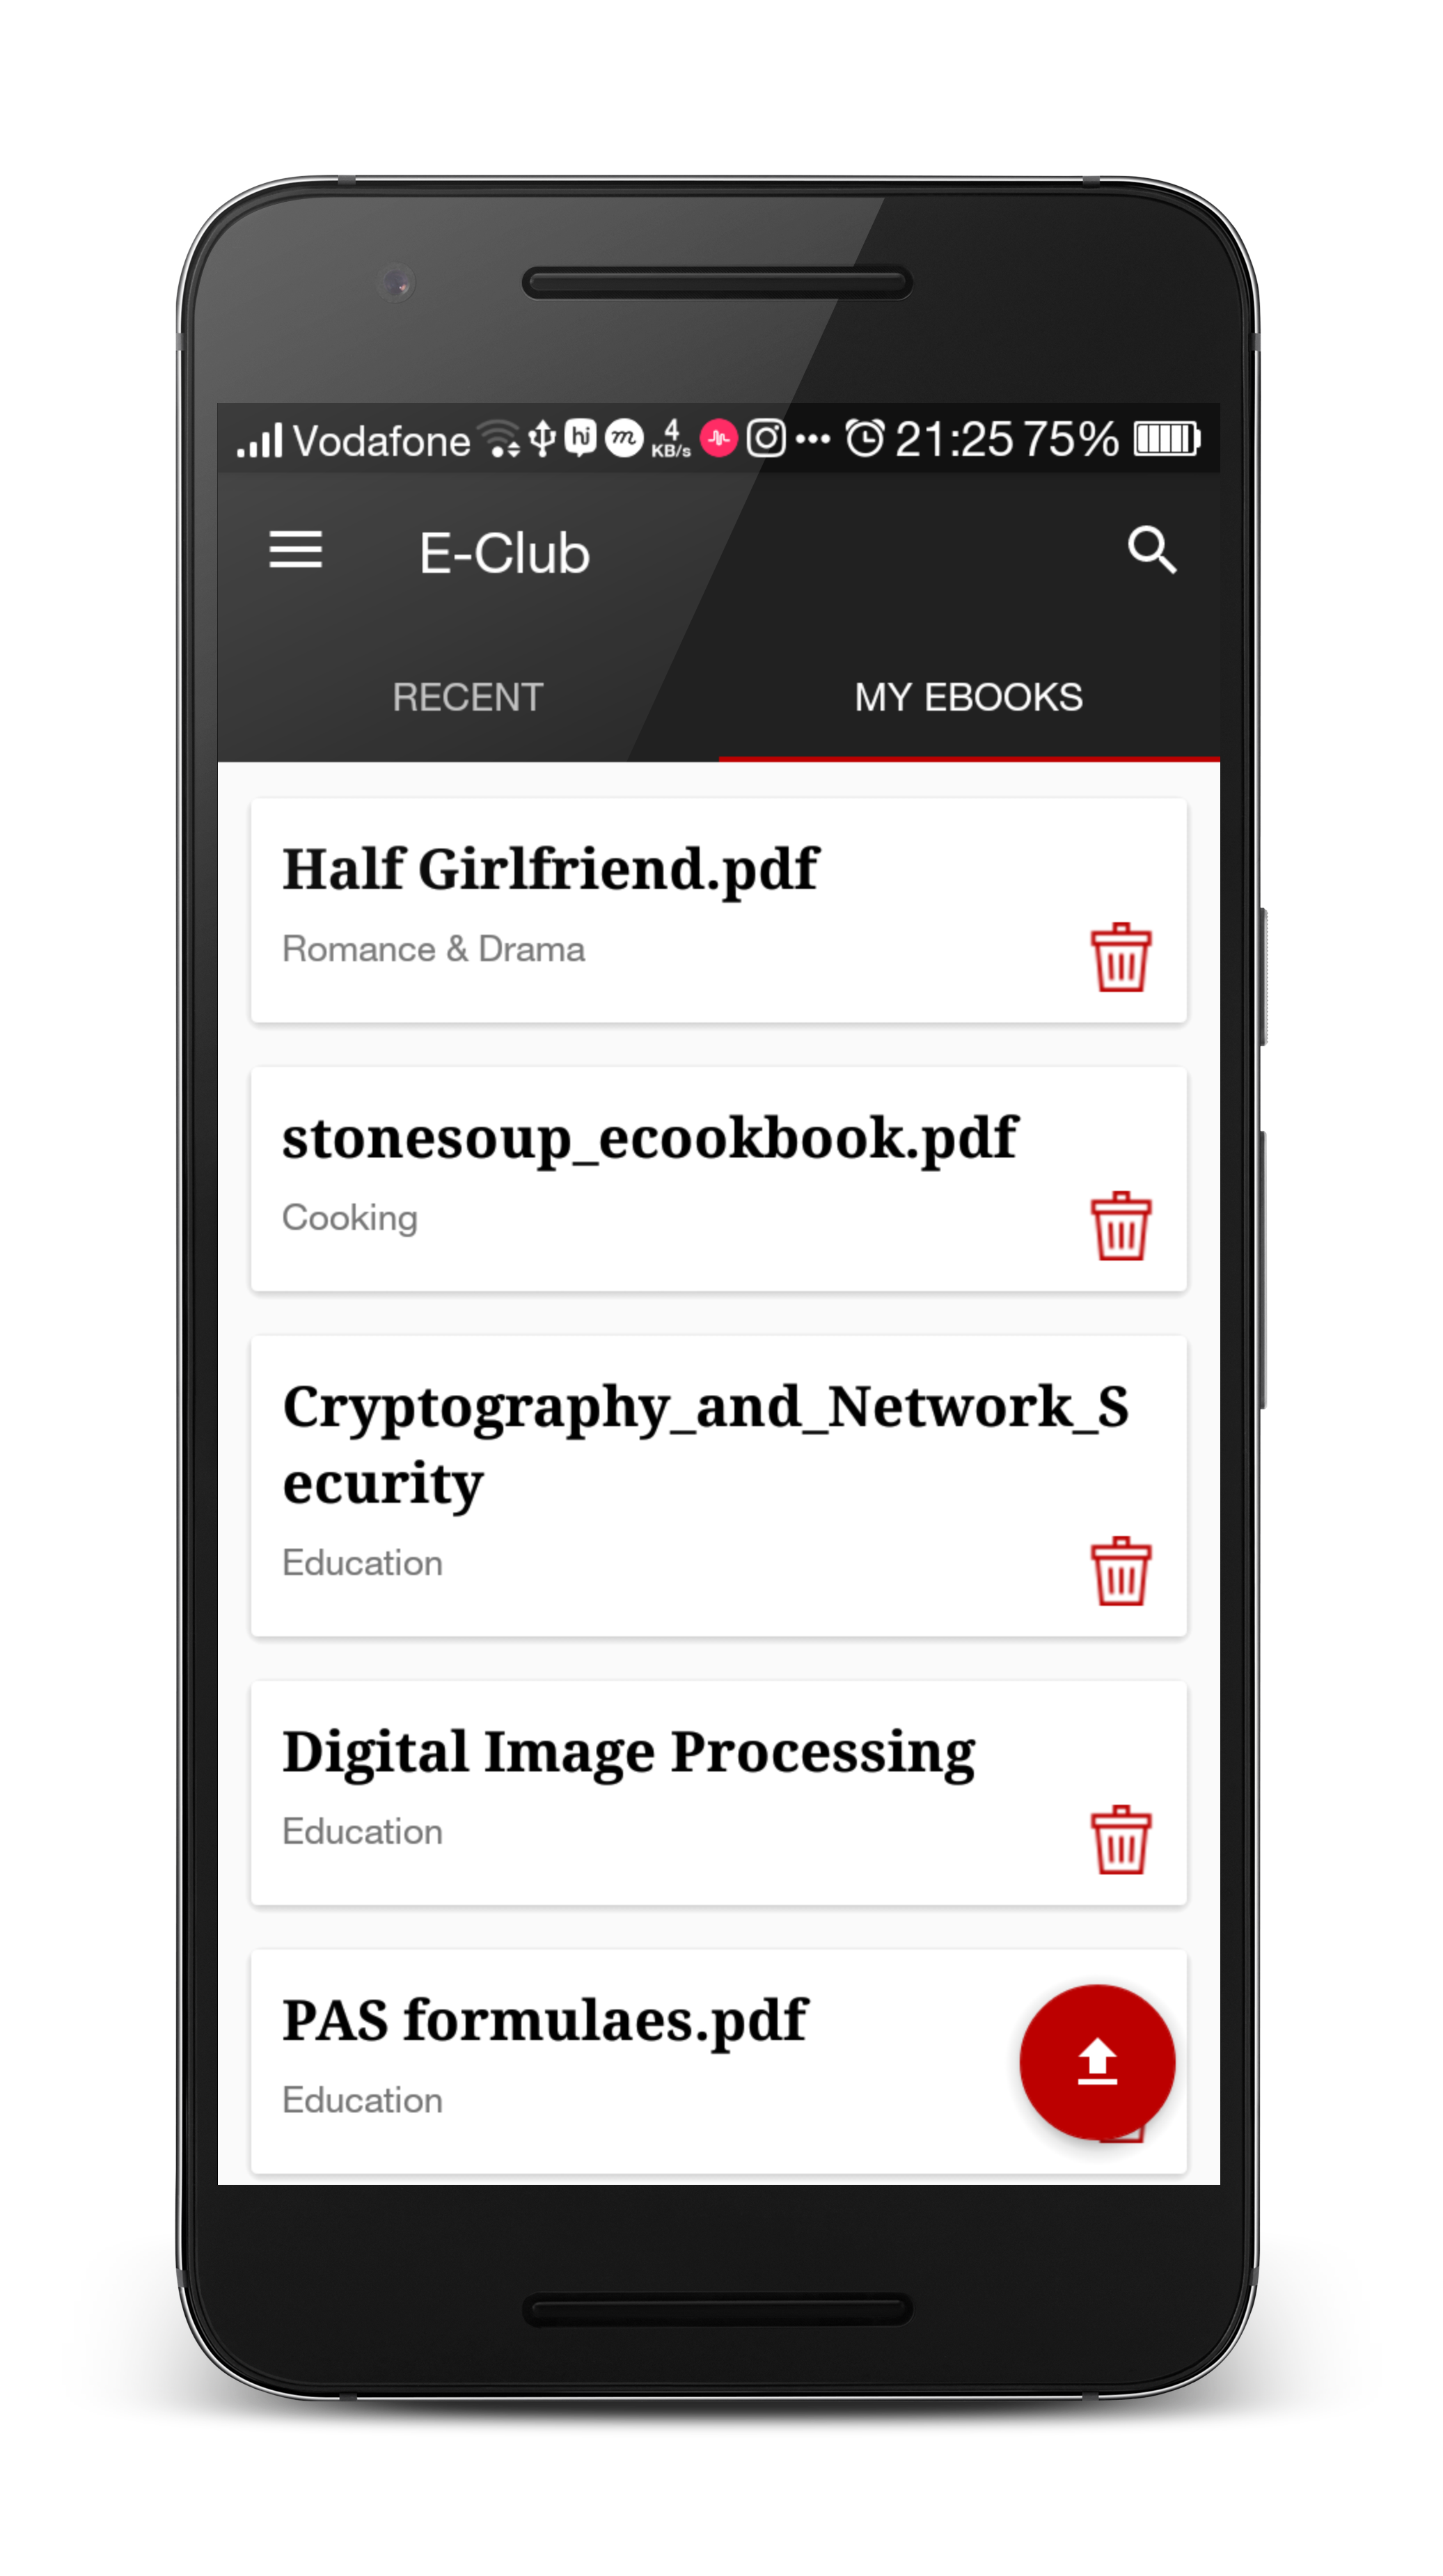
\includegraphics[scale=0.13]{images/d12.png}
\caption{Screen 6}
\end{figure}

\newpage

\begin{figure}[ht]
\centering
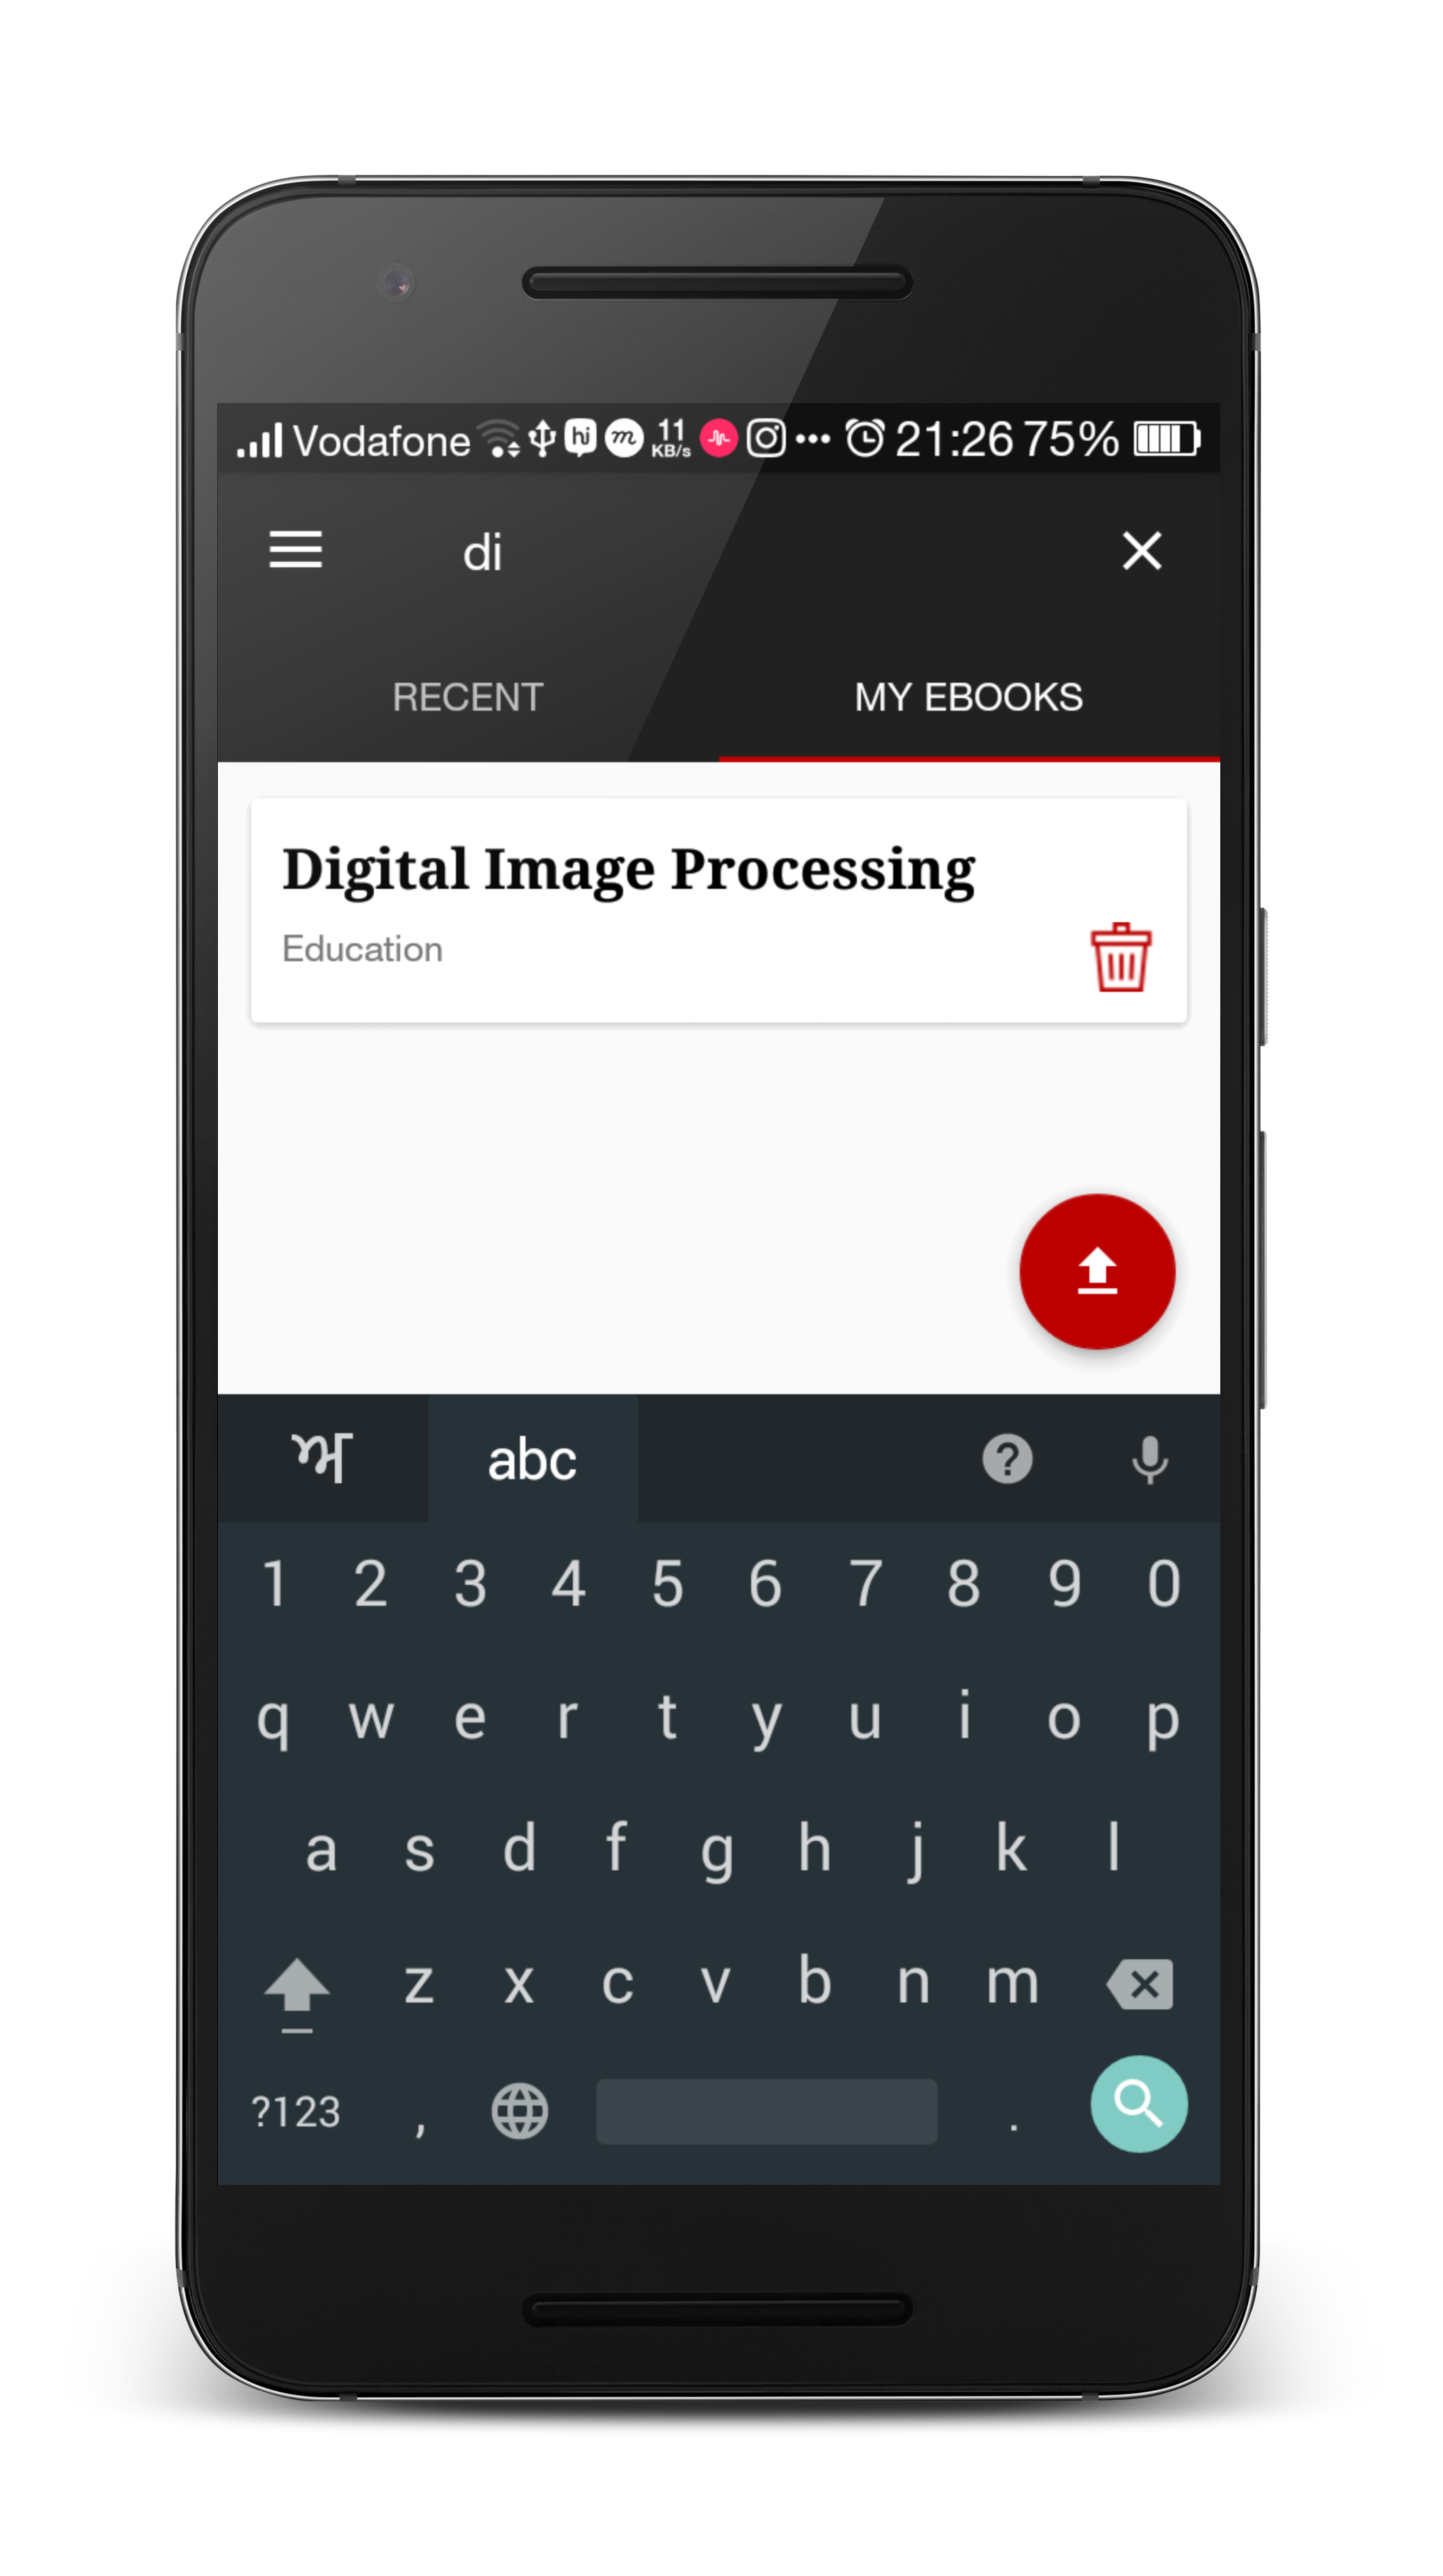
\includegraphics[scale=0.13]{images/d11.png}
\caption{Screen 7}
\end{figure}

\newpage

\begin{figure}[ht]
\centering
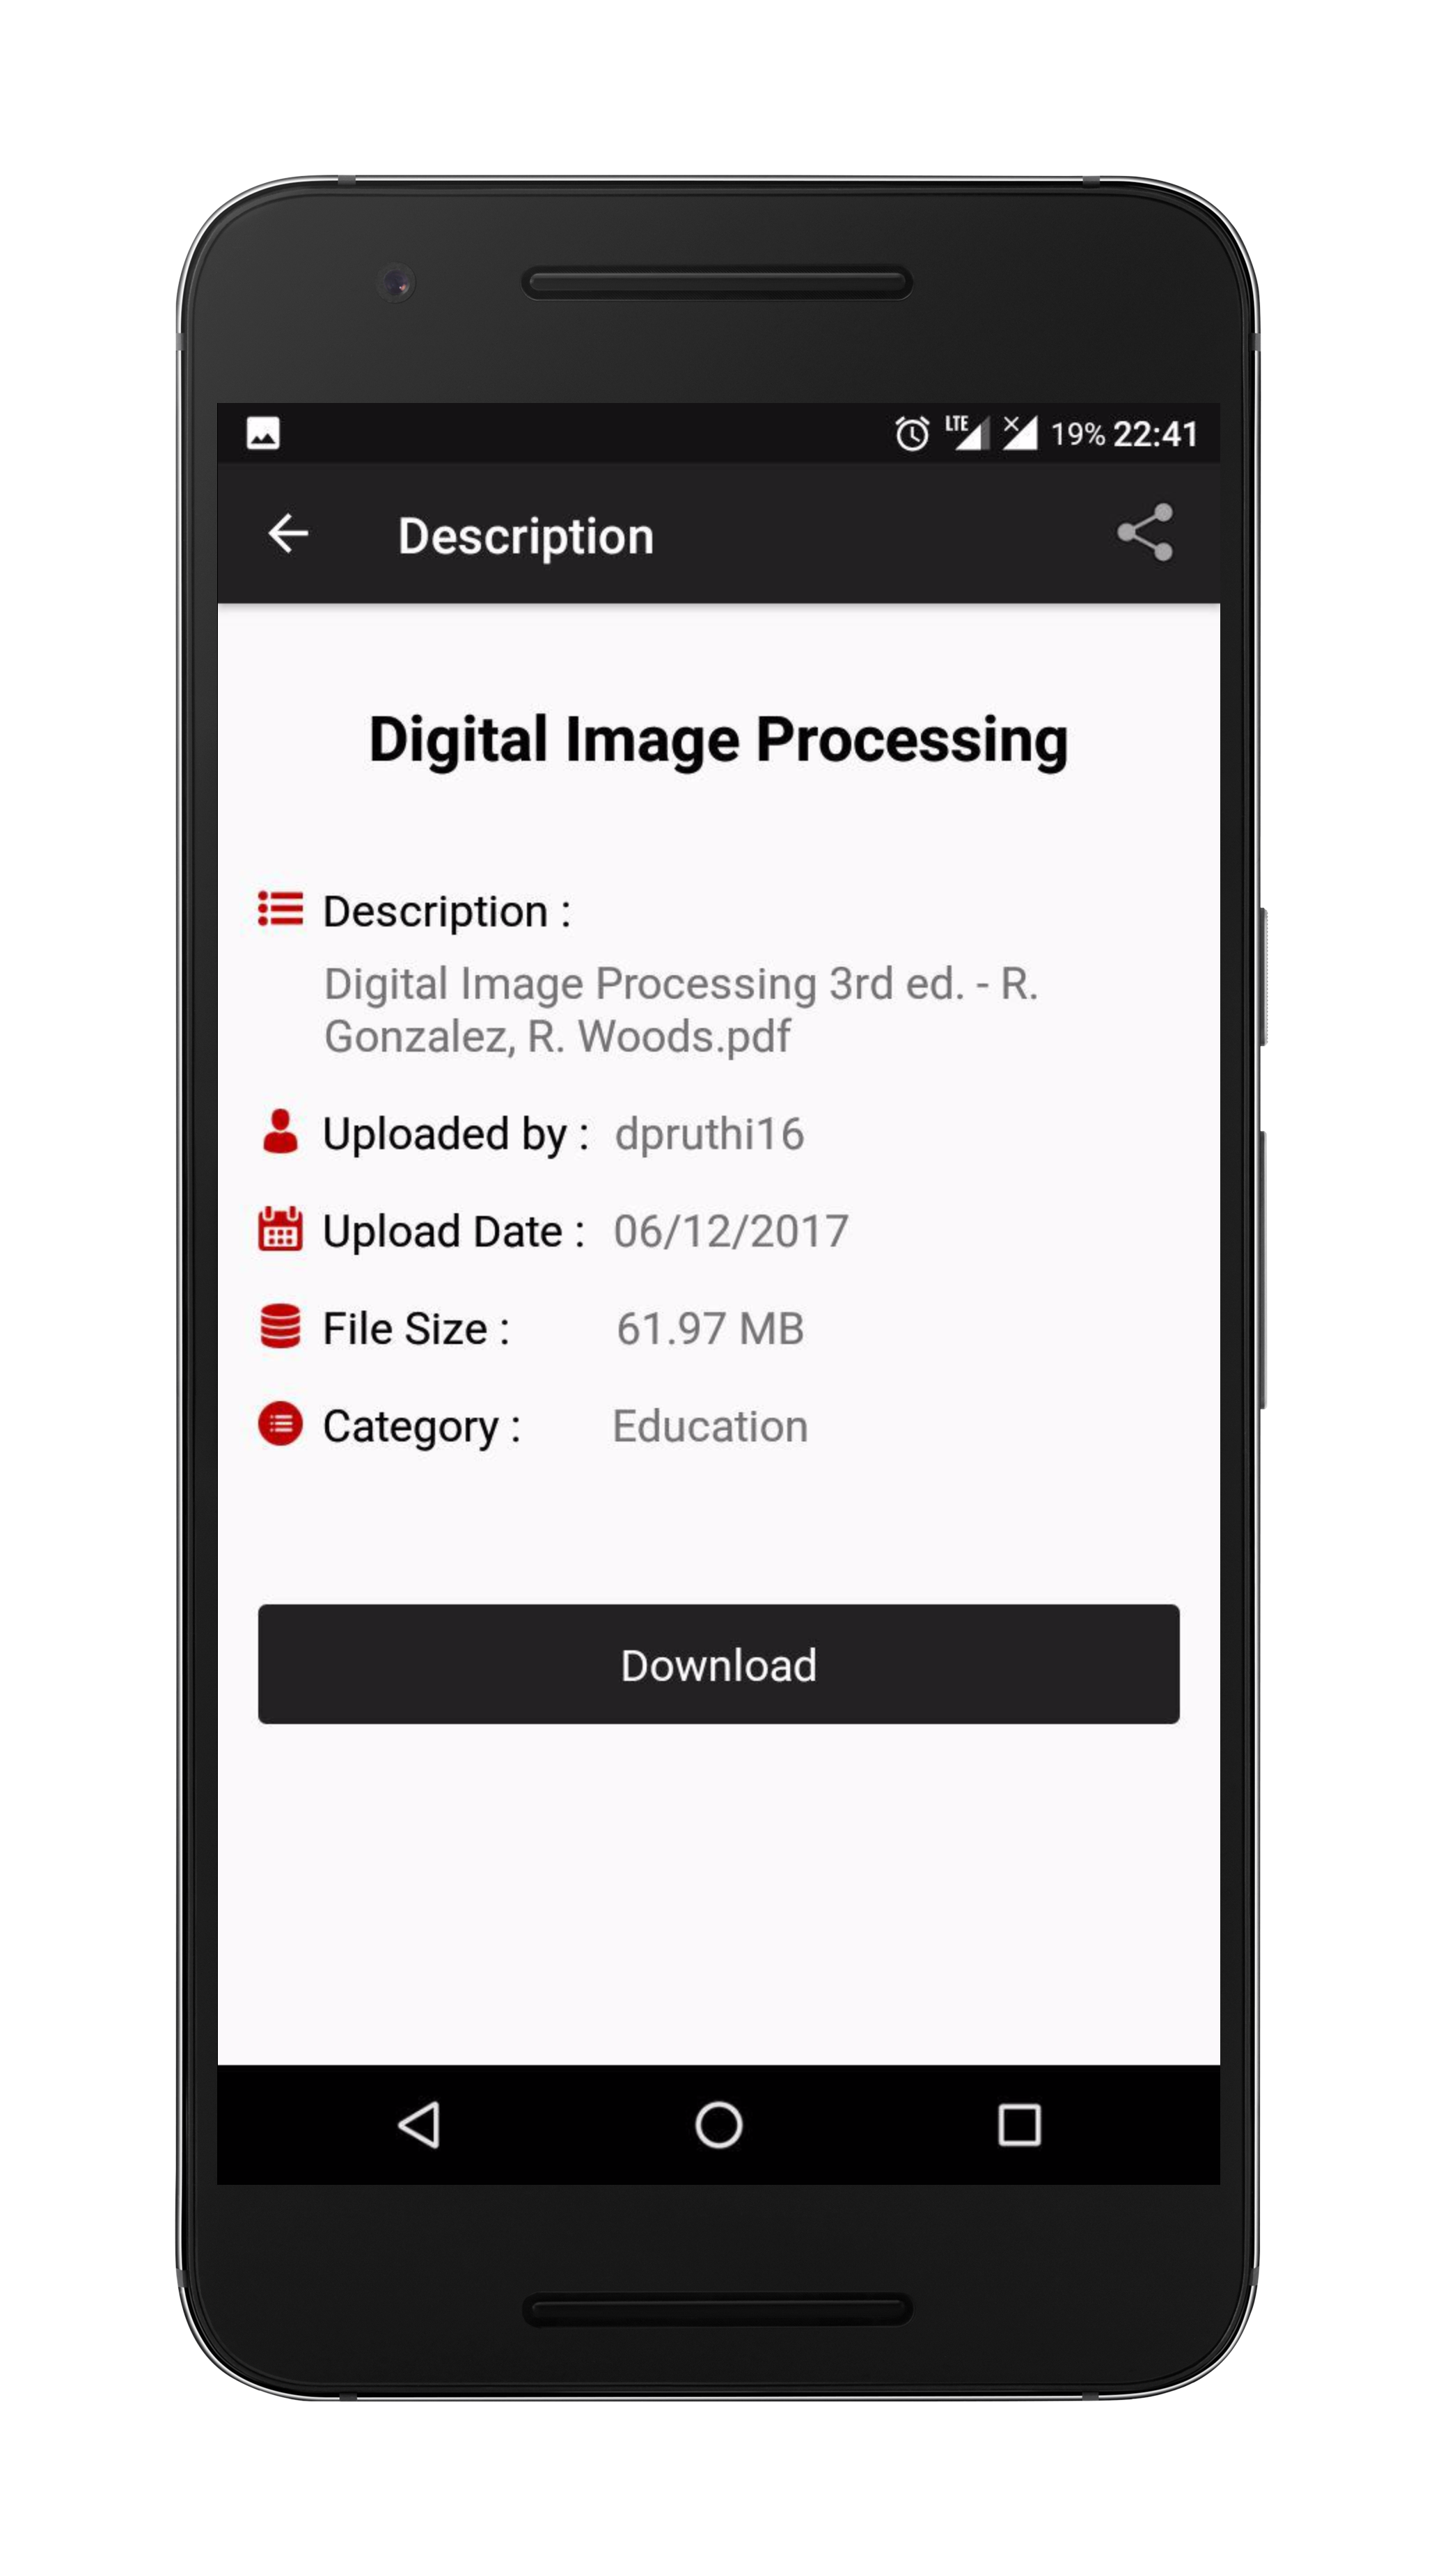
\includegraphics[scale=0.13]{images/de.png}
\caption{Screen 8}
\end{figure}

\newpage

\begin{figure}[ht]
\centering
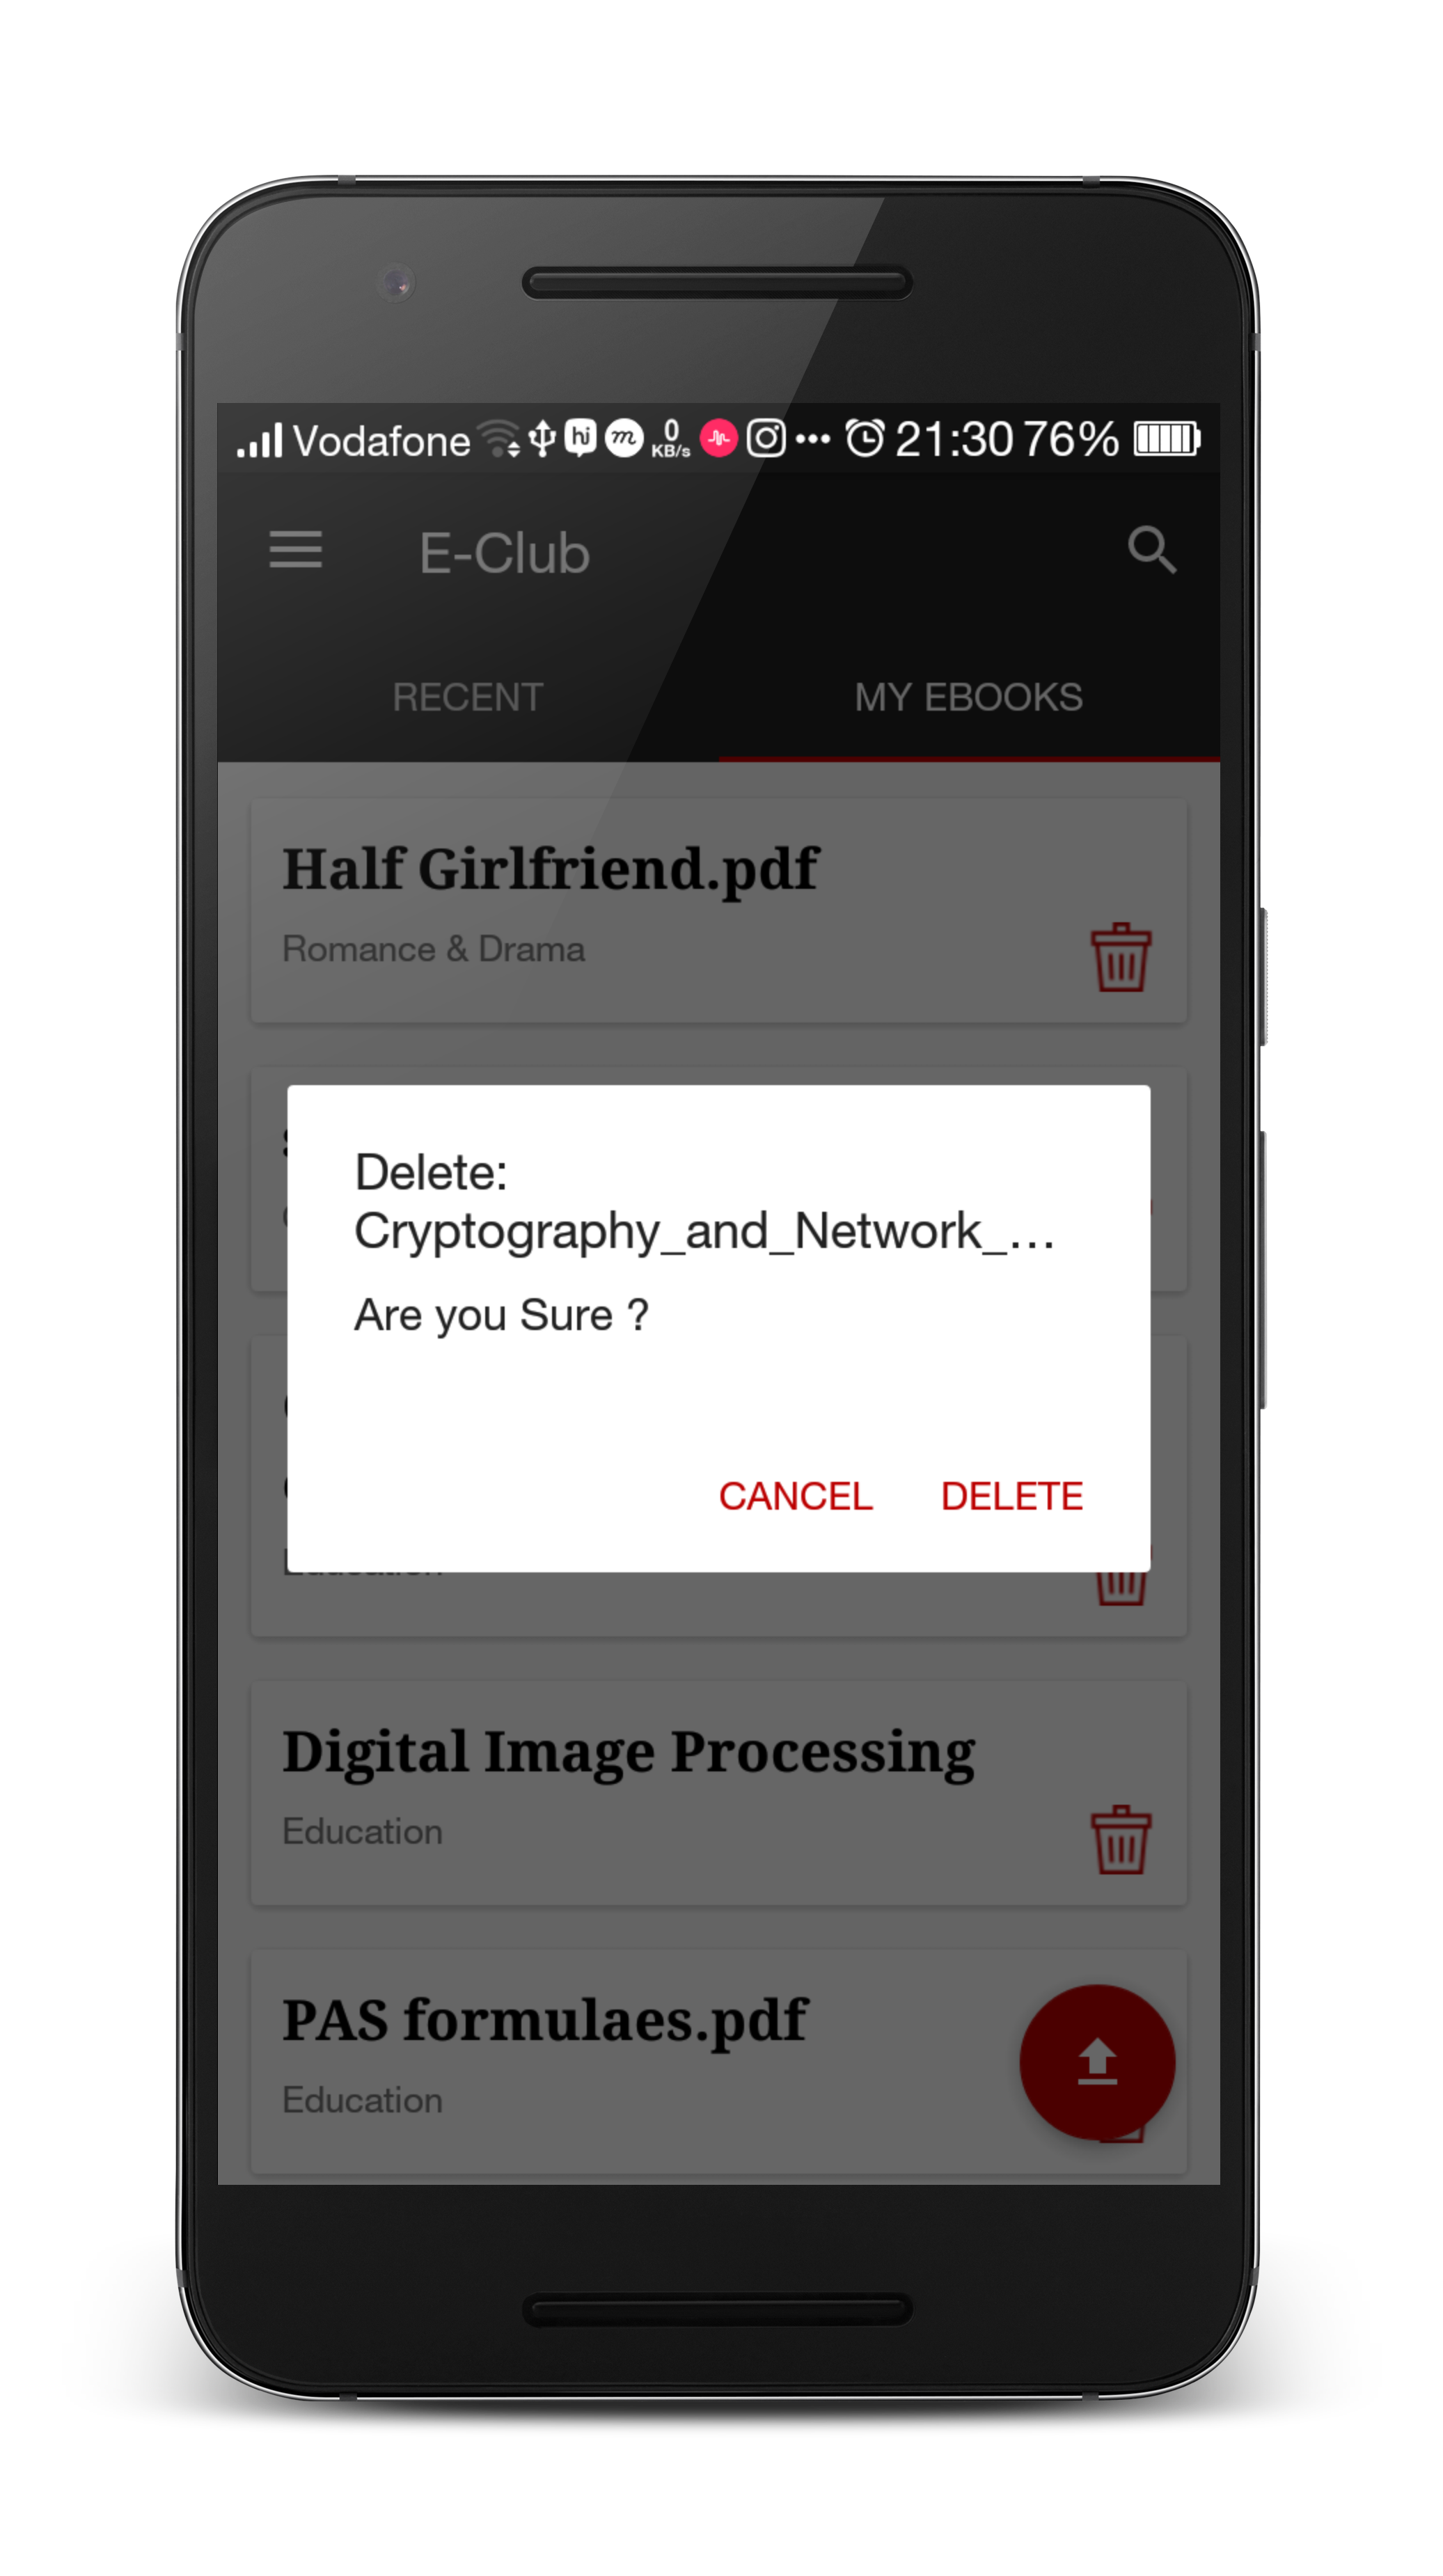
\includegraphics[scale=0.13]{images/d1.png}
\caption{Screen 9}
\end{figure}

\newpage

\begin{figure}[ht]
\centering
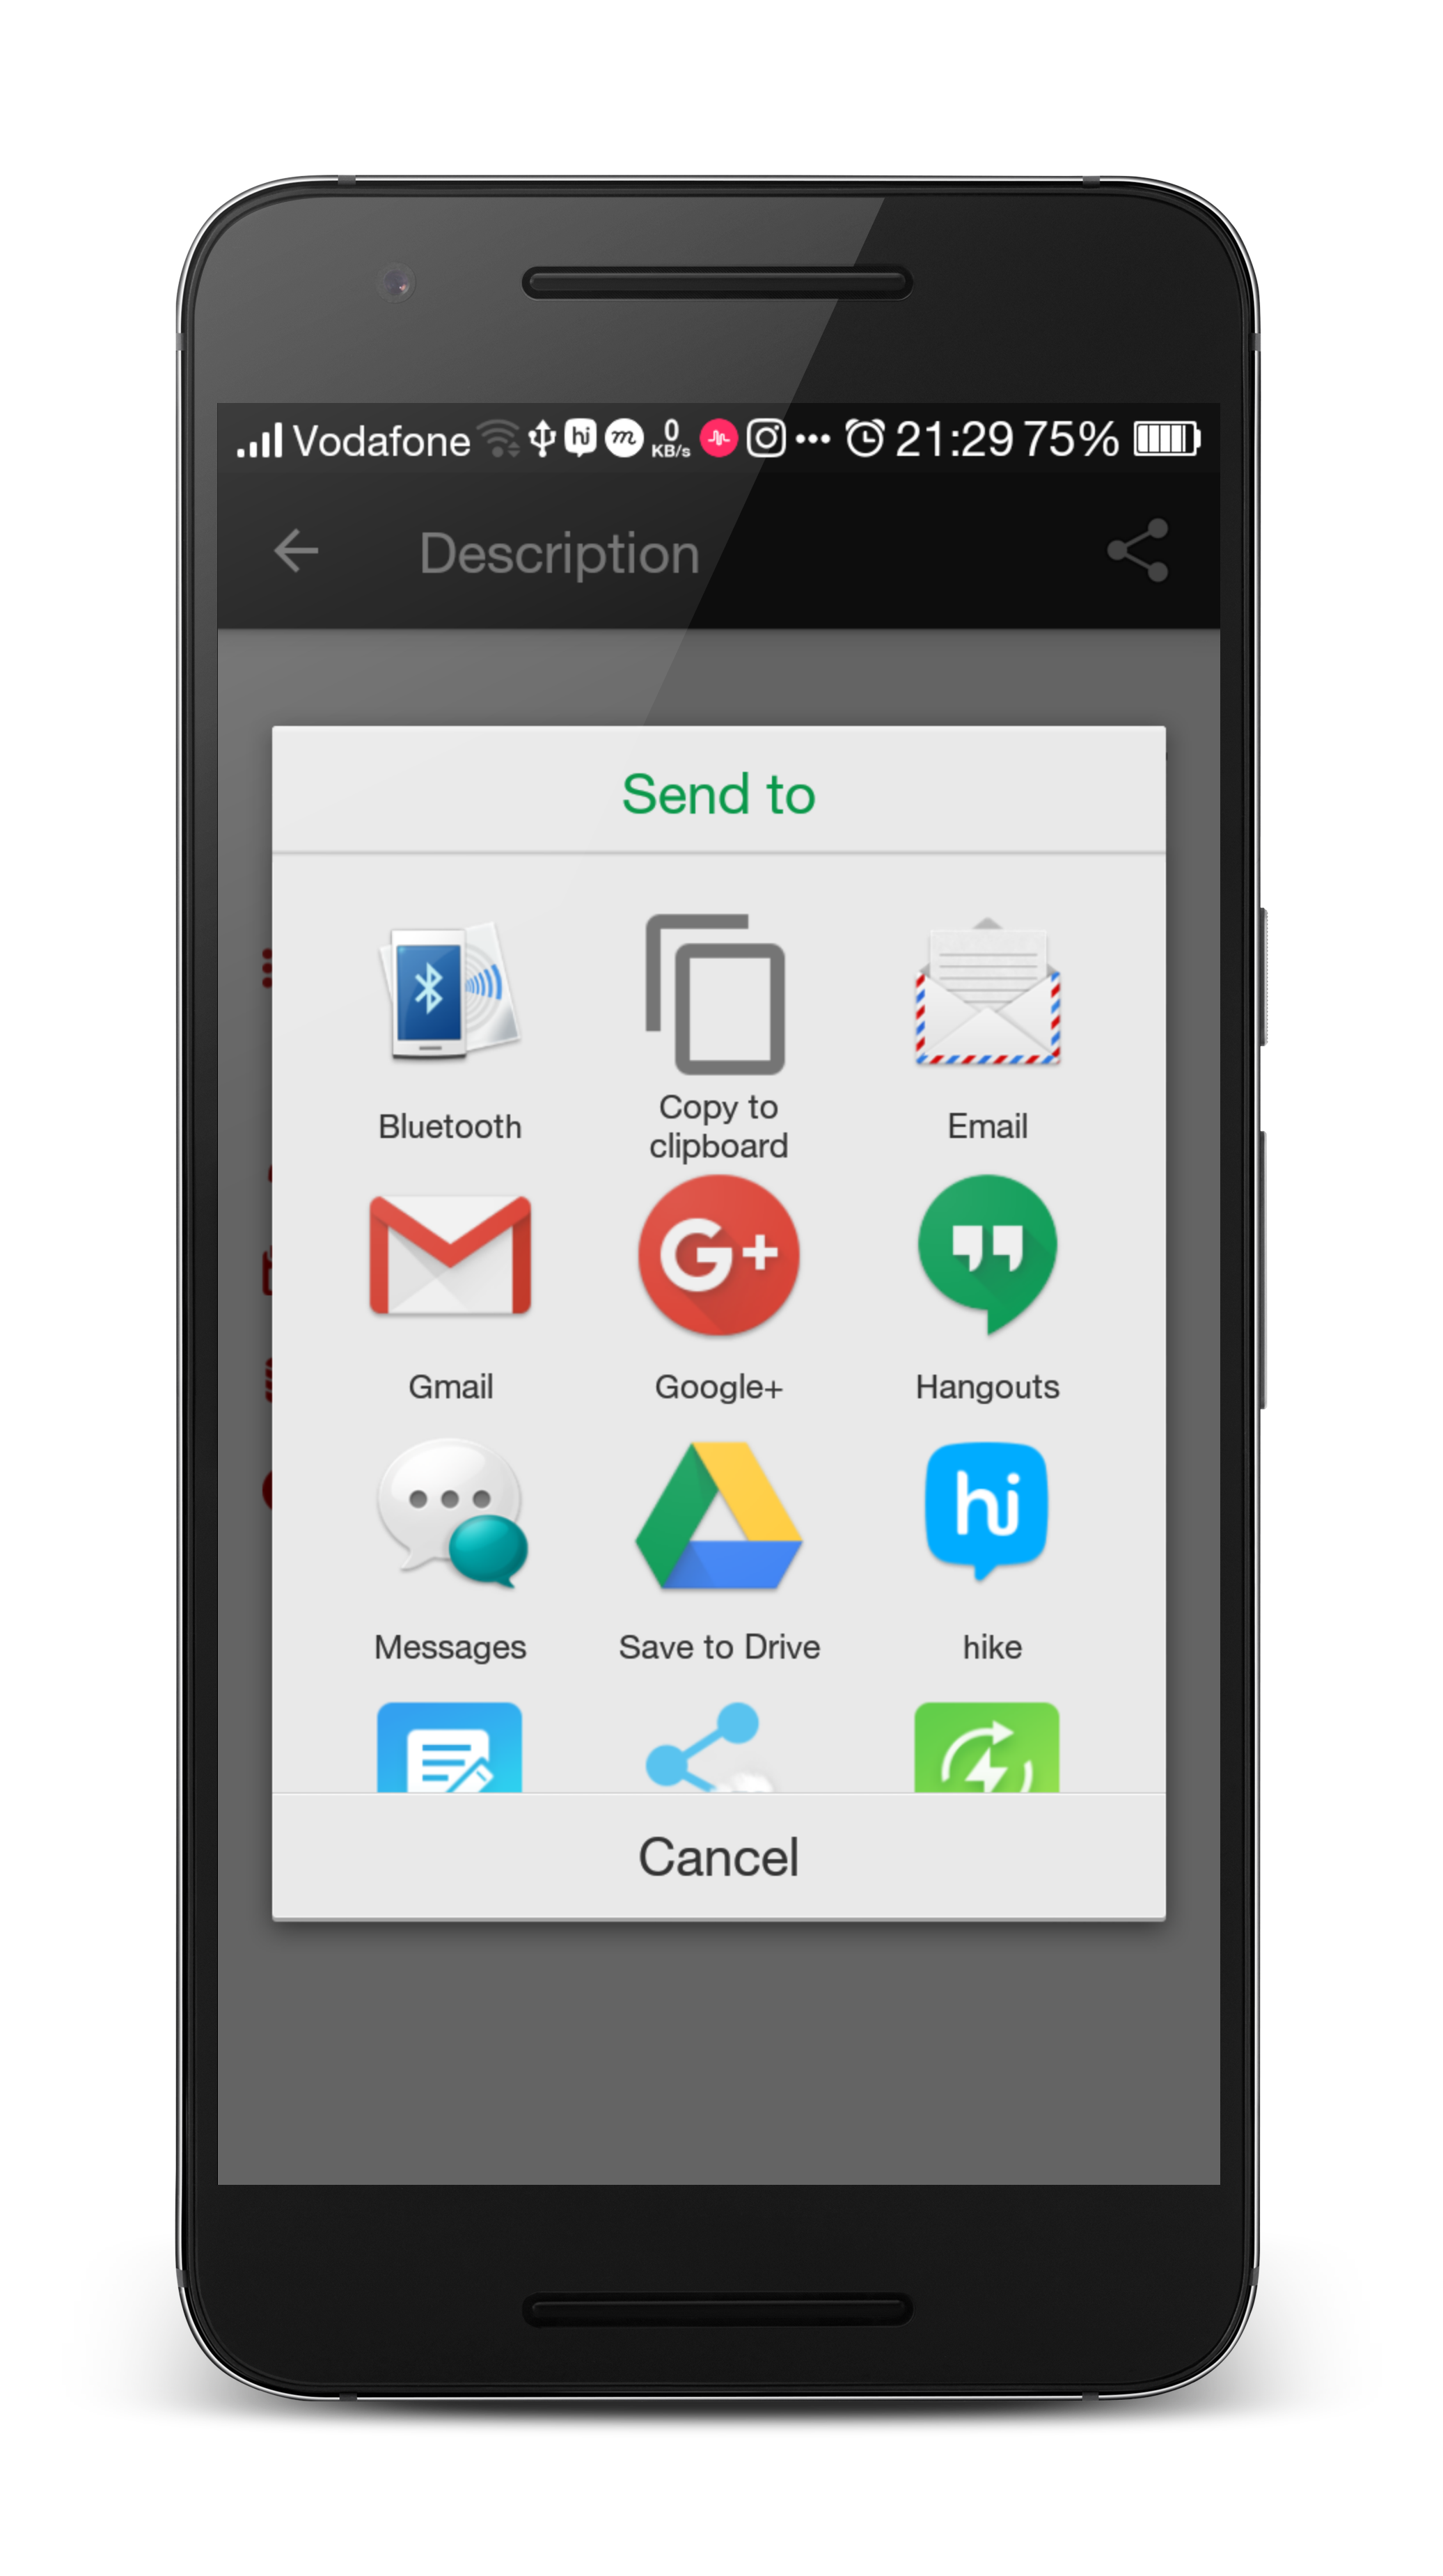
\includegraphics[scale=0.13]{images/d17.png}
\caption{Screen 10}
\end{figure}

\newpage

\begin{figure}[ht]
\centering
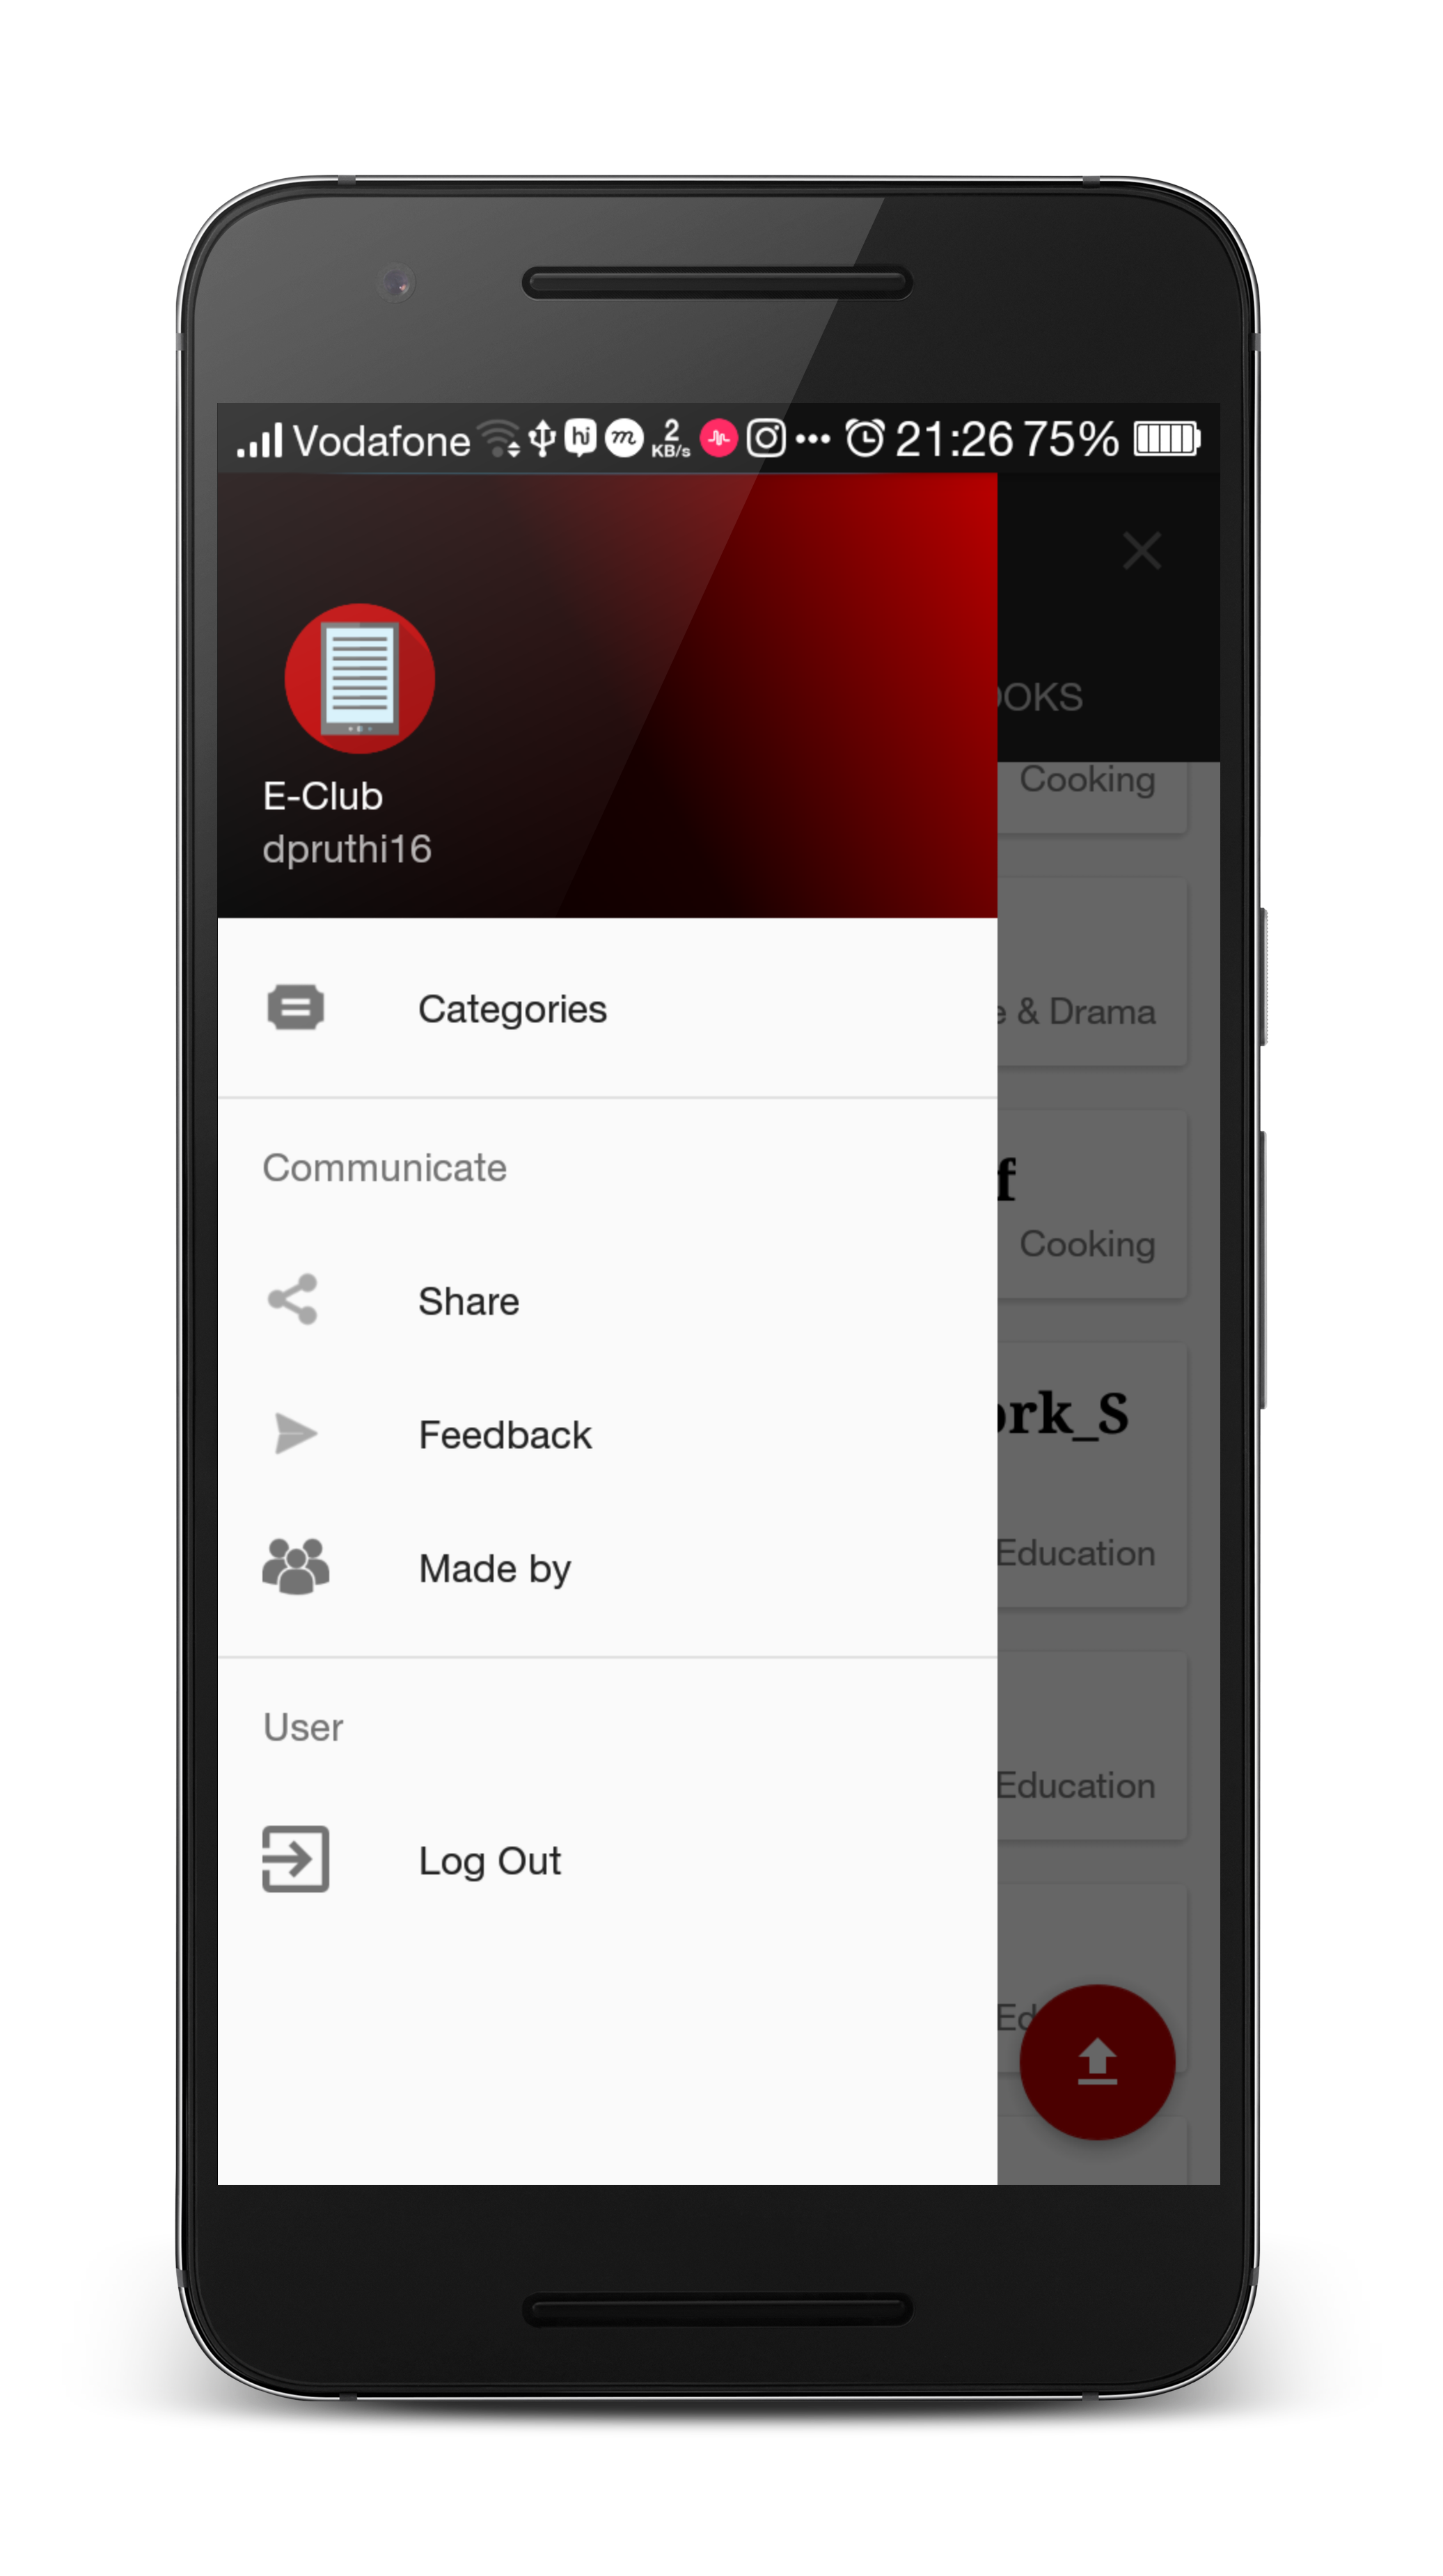
\includegraphics[scale=0.1]{images/d9.png}
\caption{Screen 11}
\end{figure}

\newpage

\begin{figure}[ht]
\centering
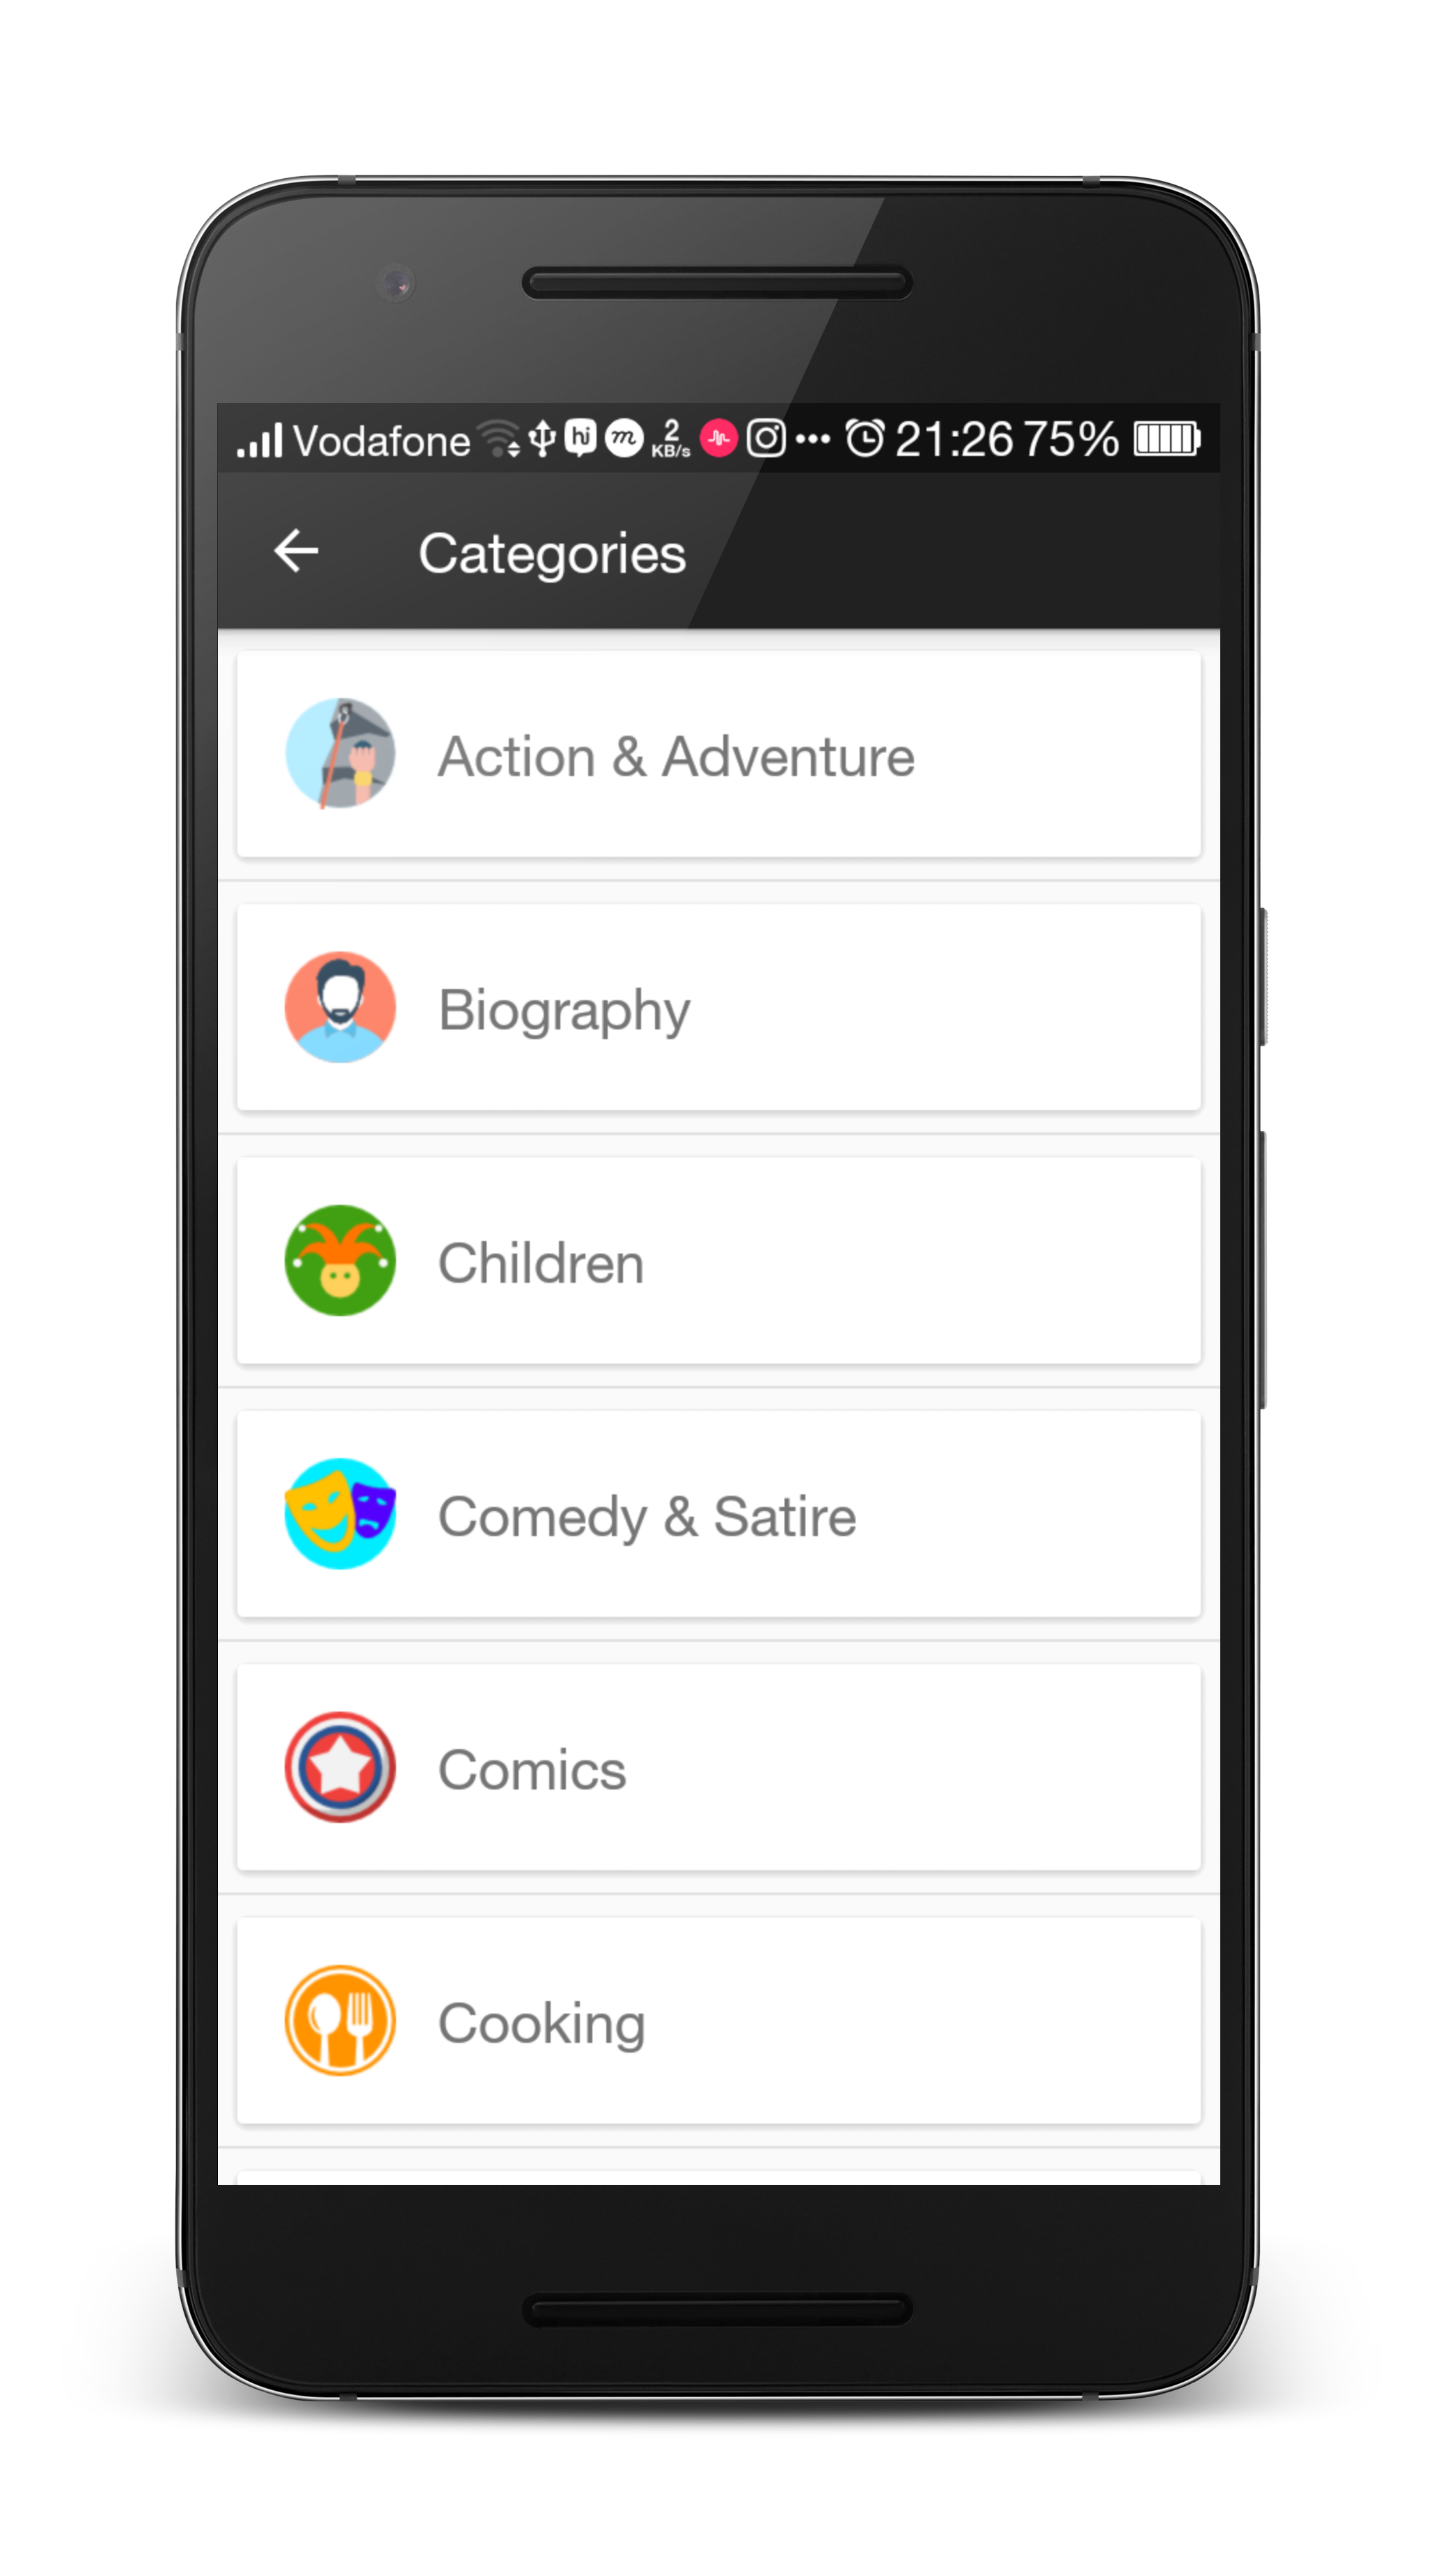
\includegraphics[scale=0.13]{images/d8.png}
\caption{Screen 12}
\end{figure}

\newpage

\begin{figure}[ht]
\centering
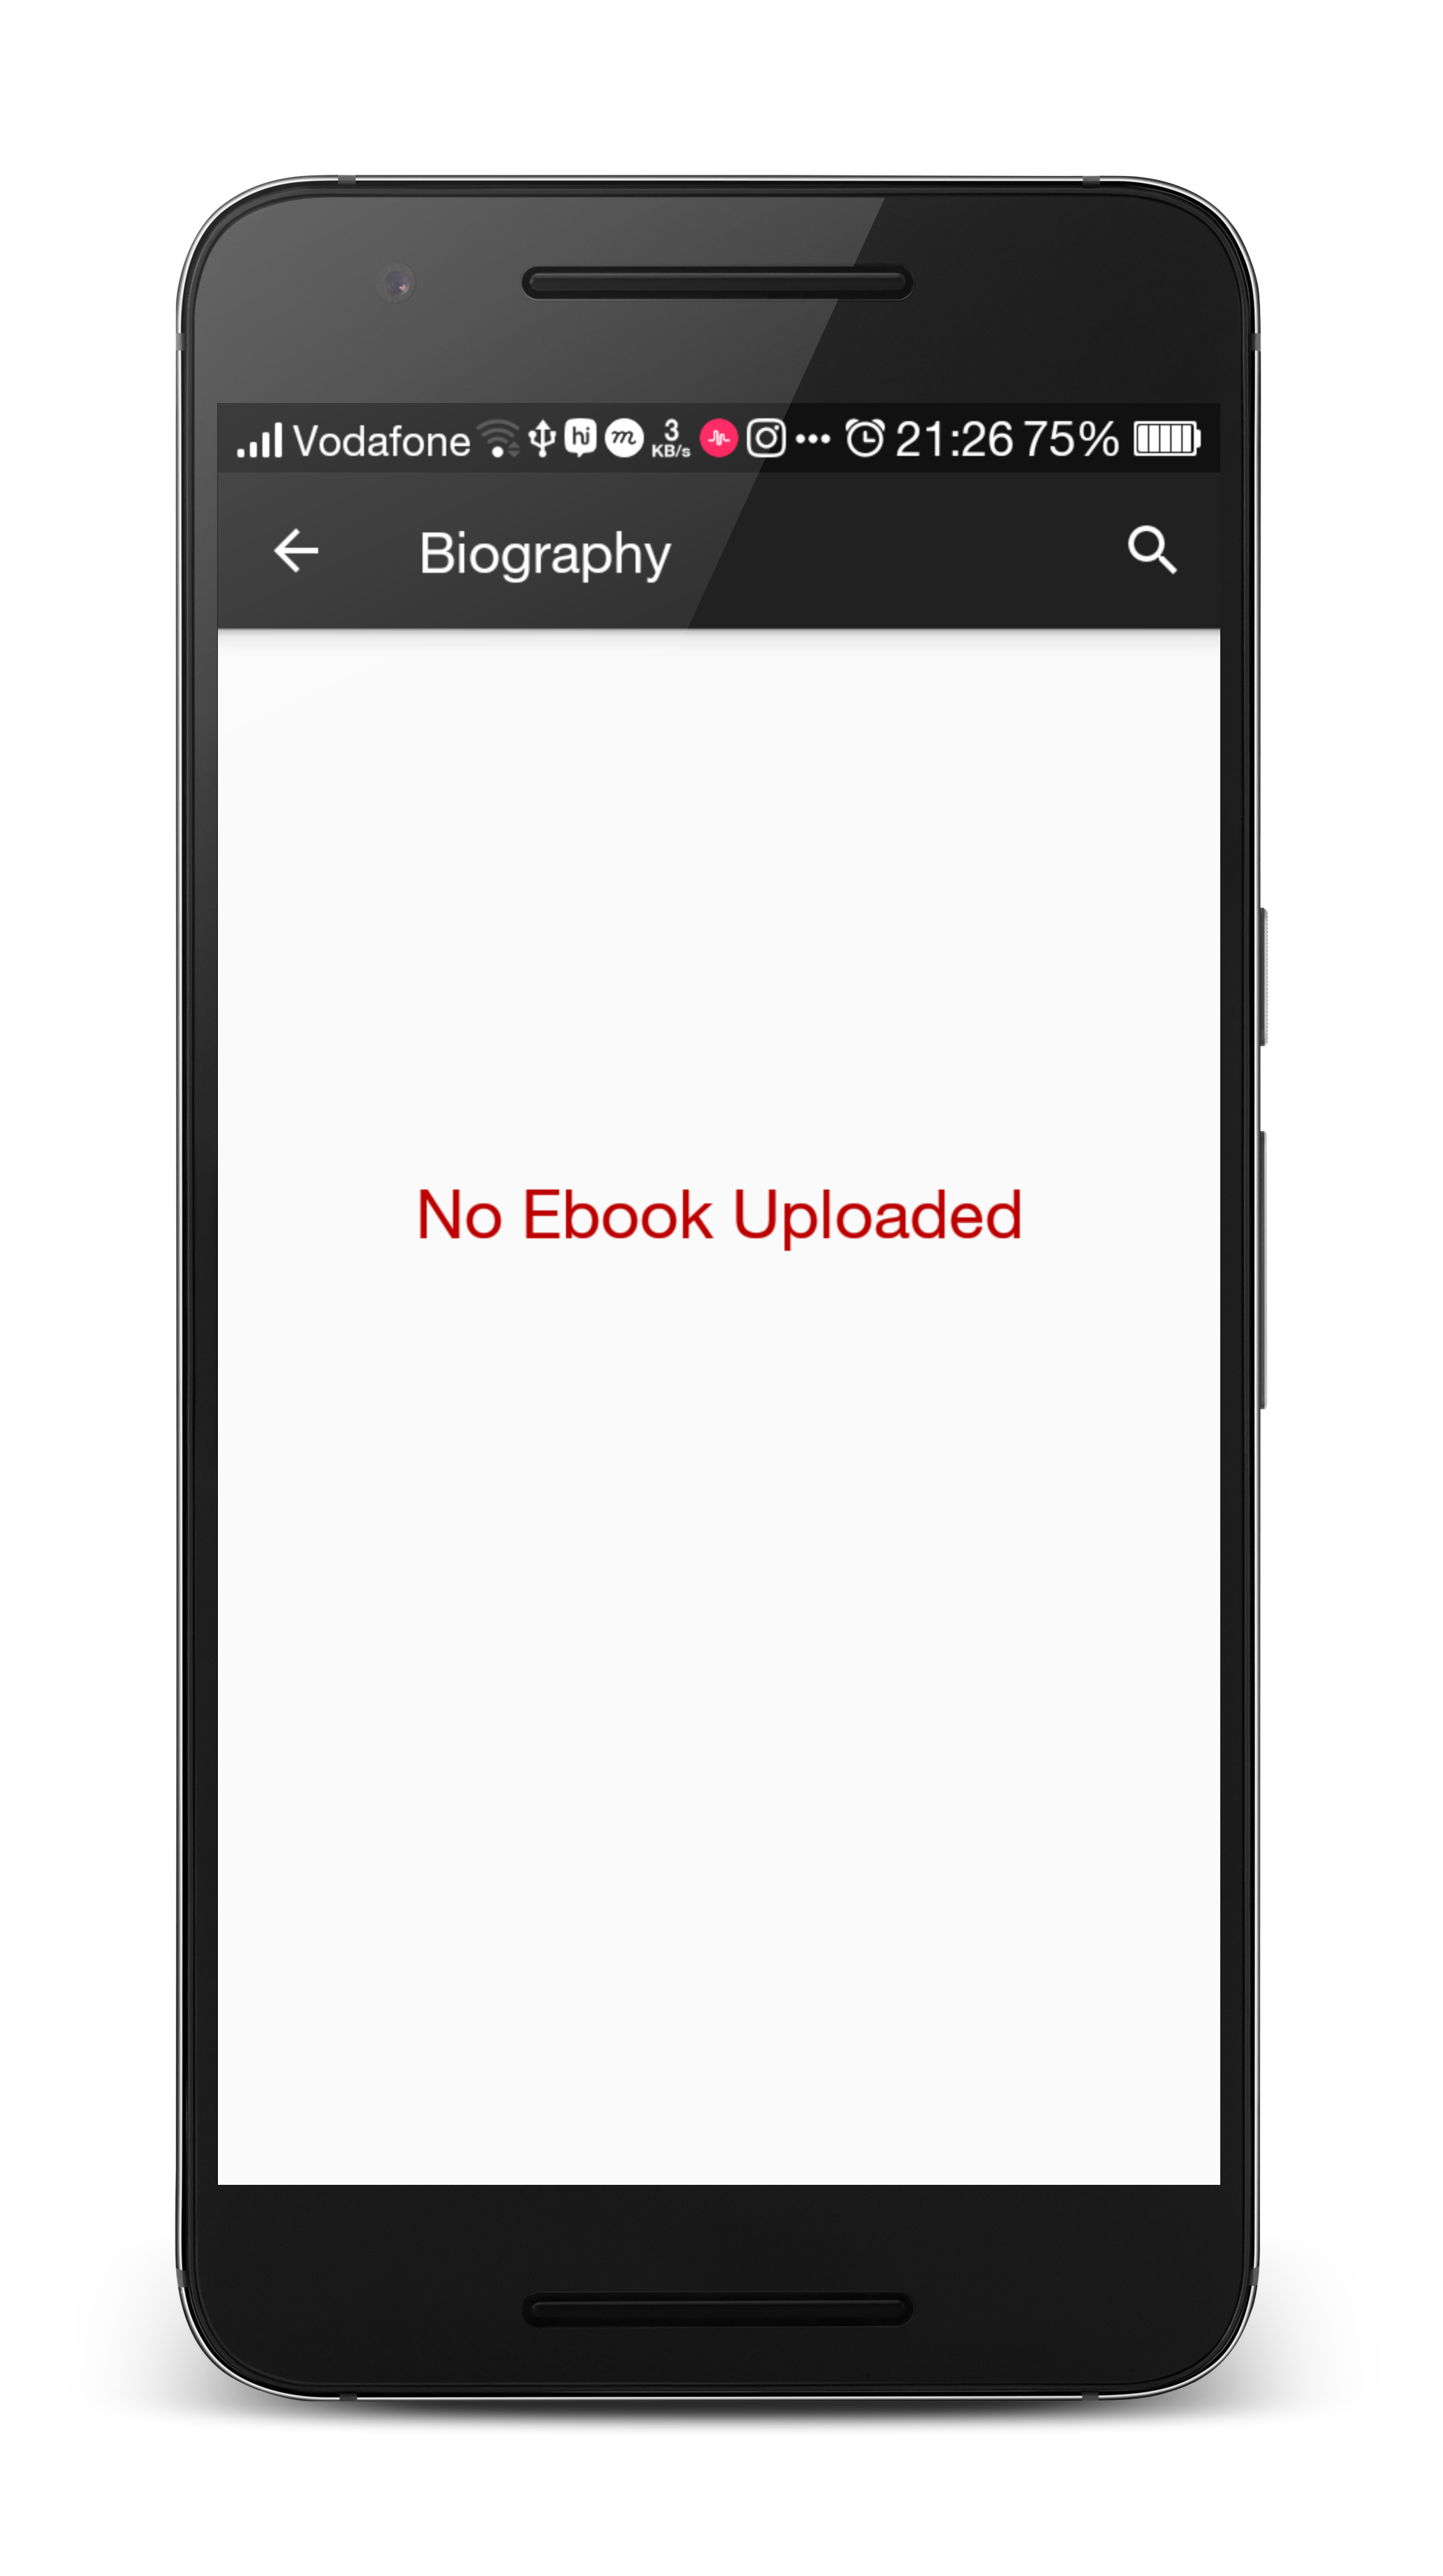
\includegraphics[scale=0.13]{images/d7.png}
\caption{Screen 13}
\end{figure}

\newpage

\begin{figure}[ht]
\centering
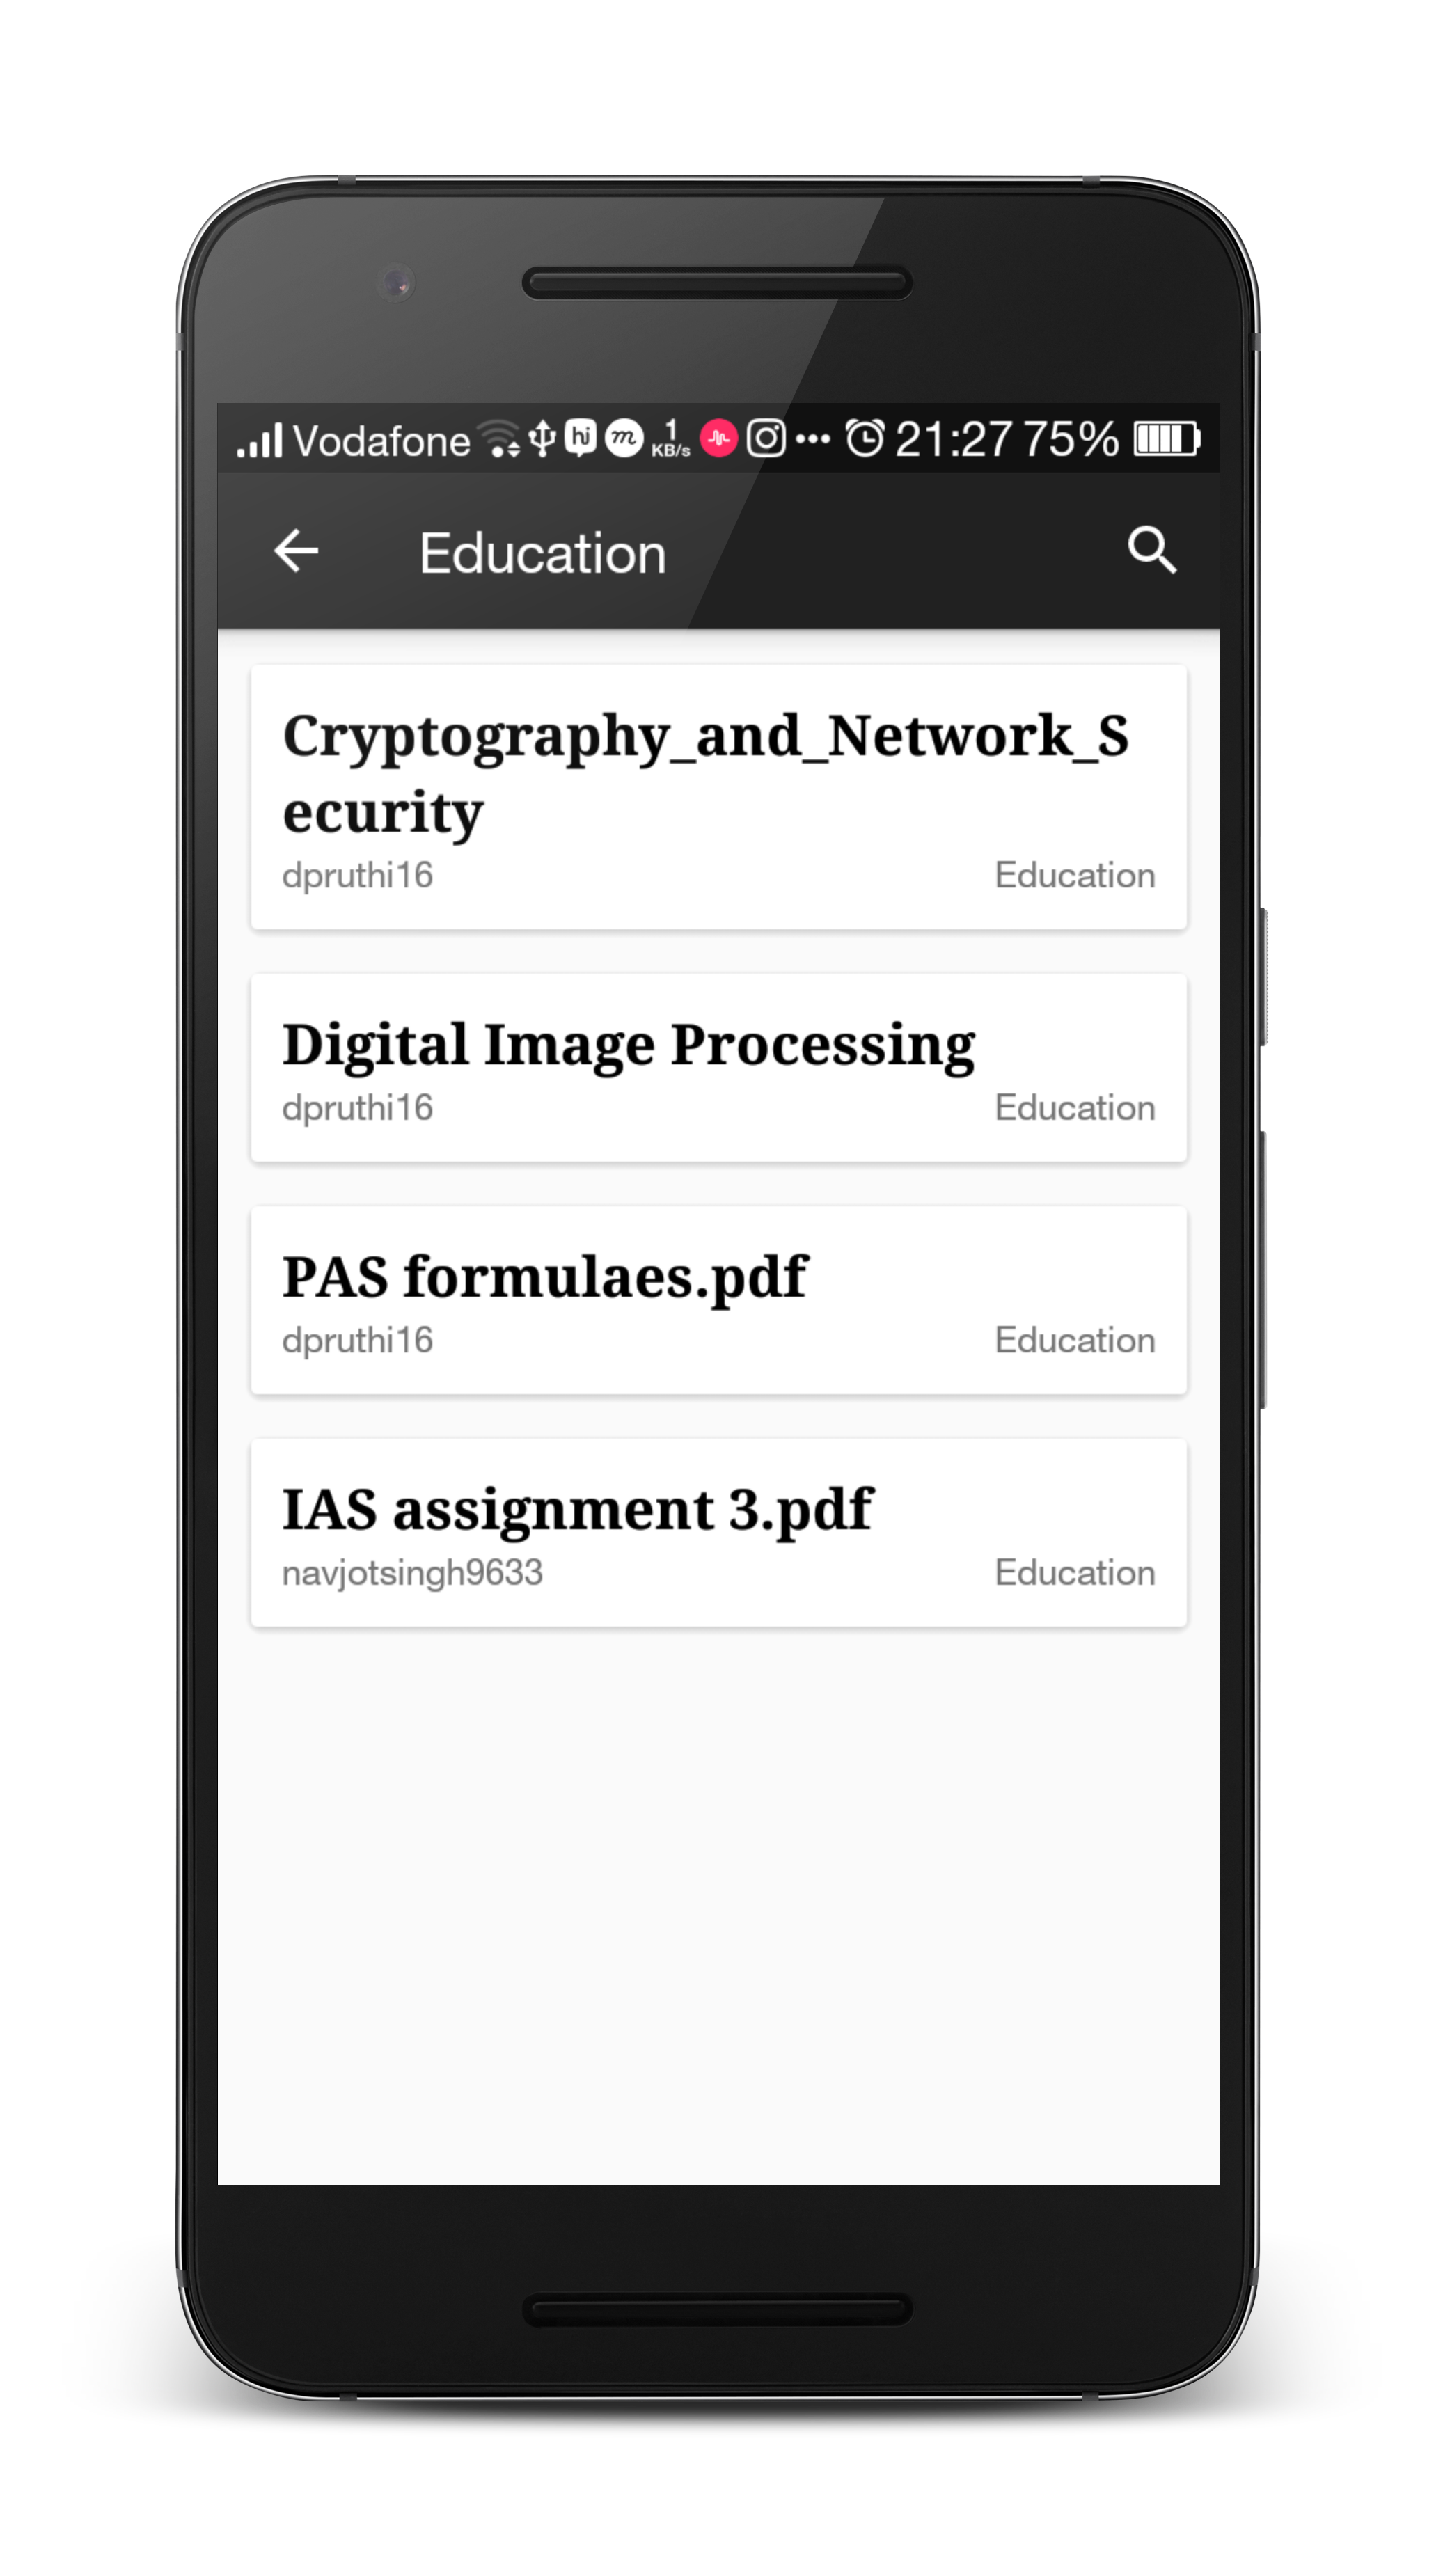
\includegraphics[scale=0.13]{images/d6.png}
\caption{Screen 14}
\end{figure}

\newpage
\begin{figure}[ht]
\centering
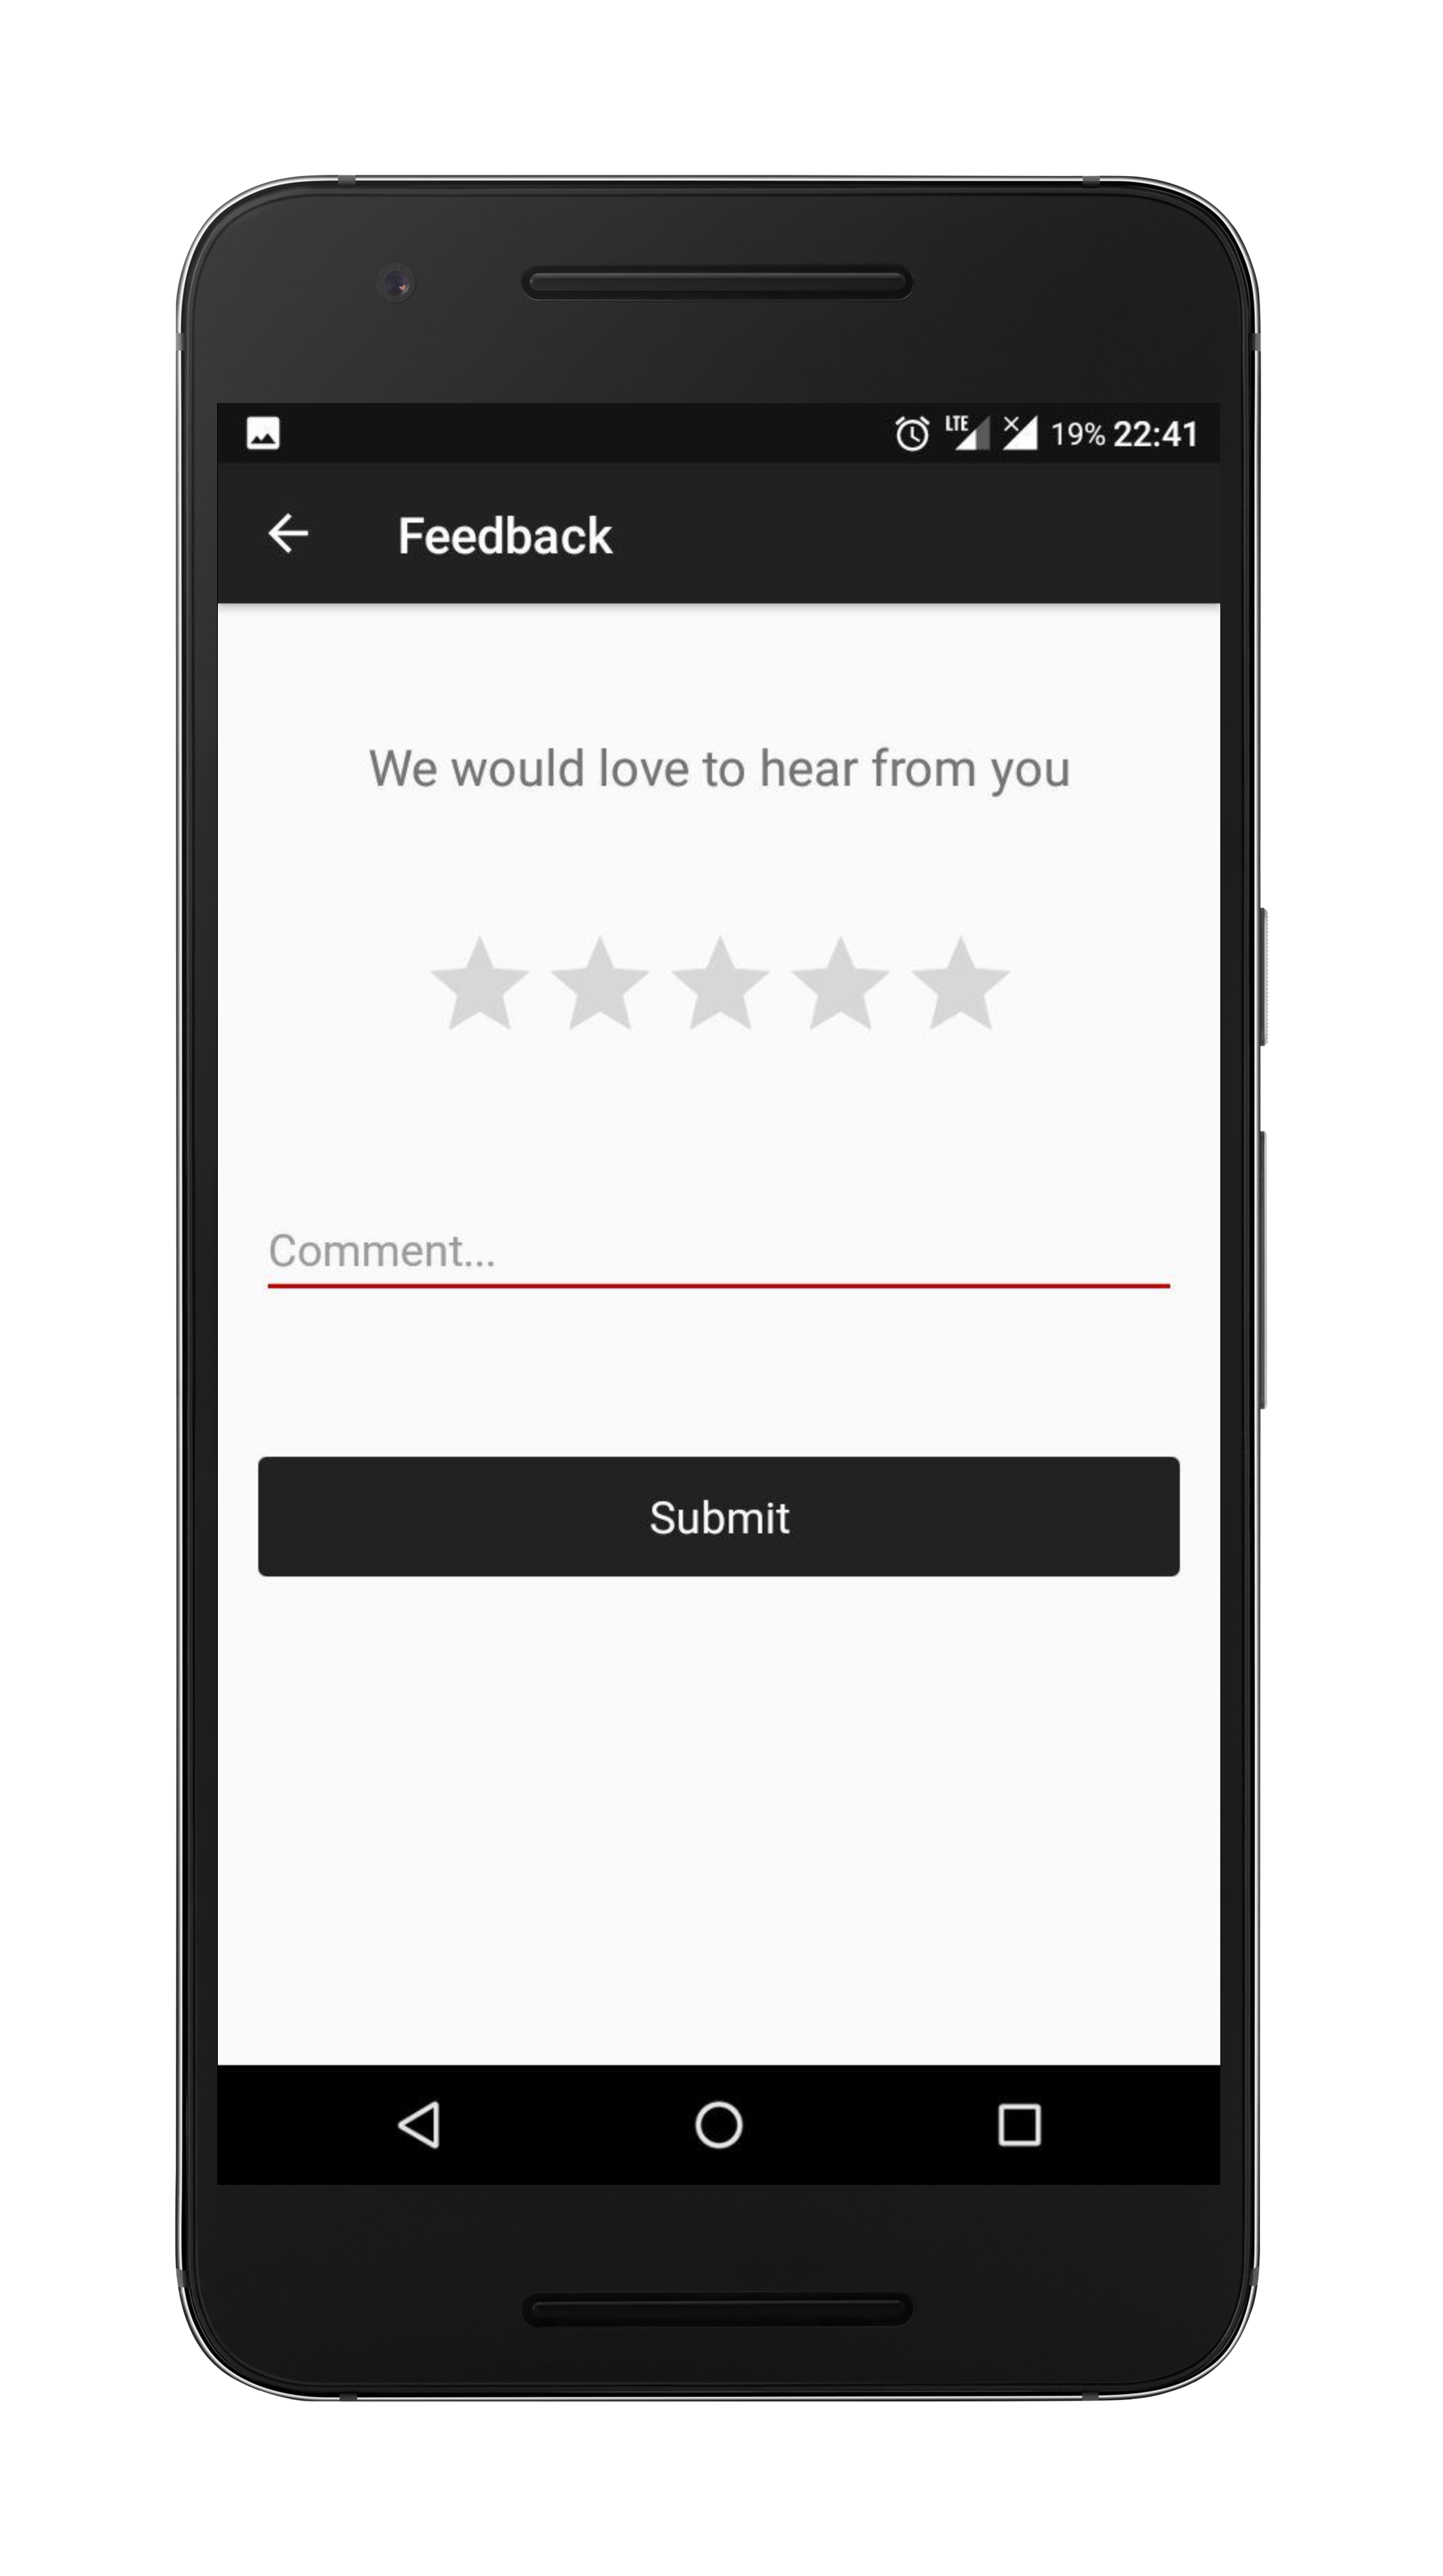
\includegraphics[scale=0.13]{images/f.png}
\caption{Screen 15}
\end{figure}

\newpage
\begin{figure}[ht]
\centering
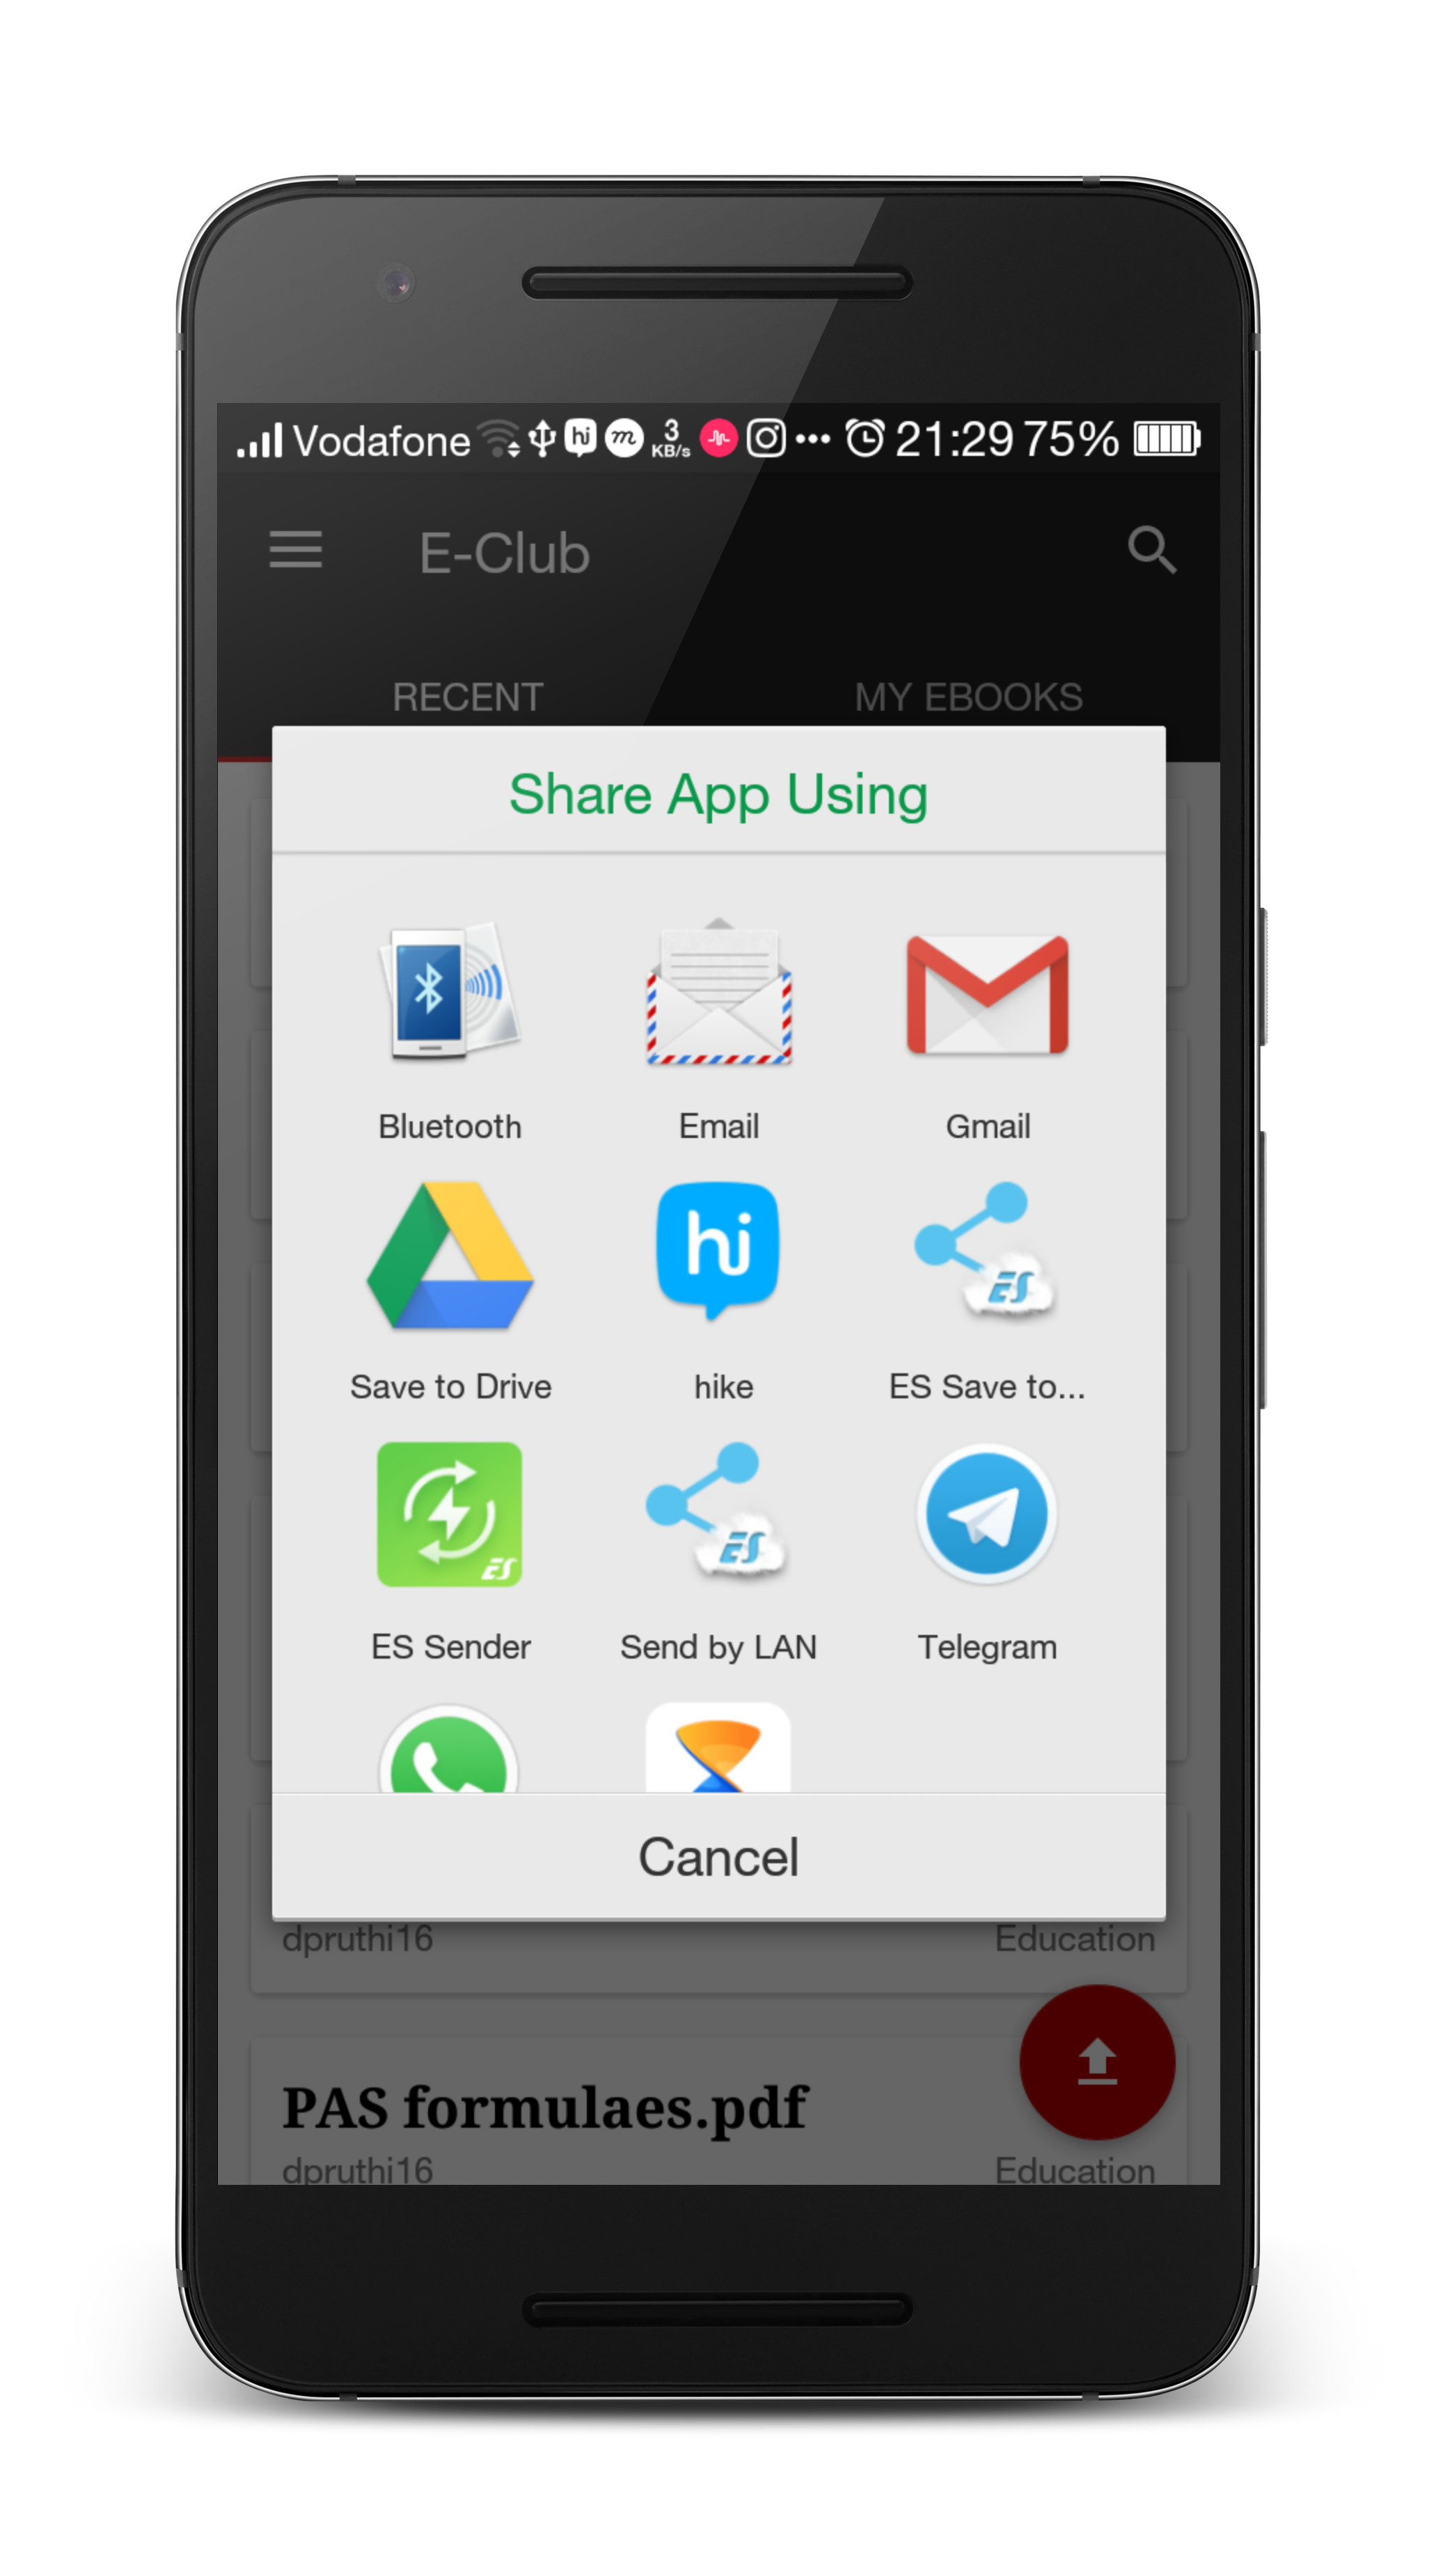
\includegraphics[scale=0.13]{images/d4.png}
\caption{Screen 16}
\end{figure}

\newpage
\begin{figure}[ht]
\centering
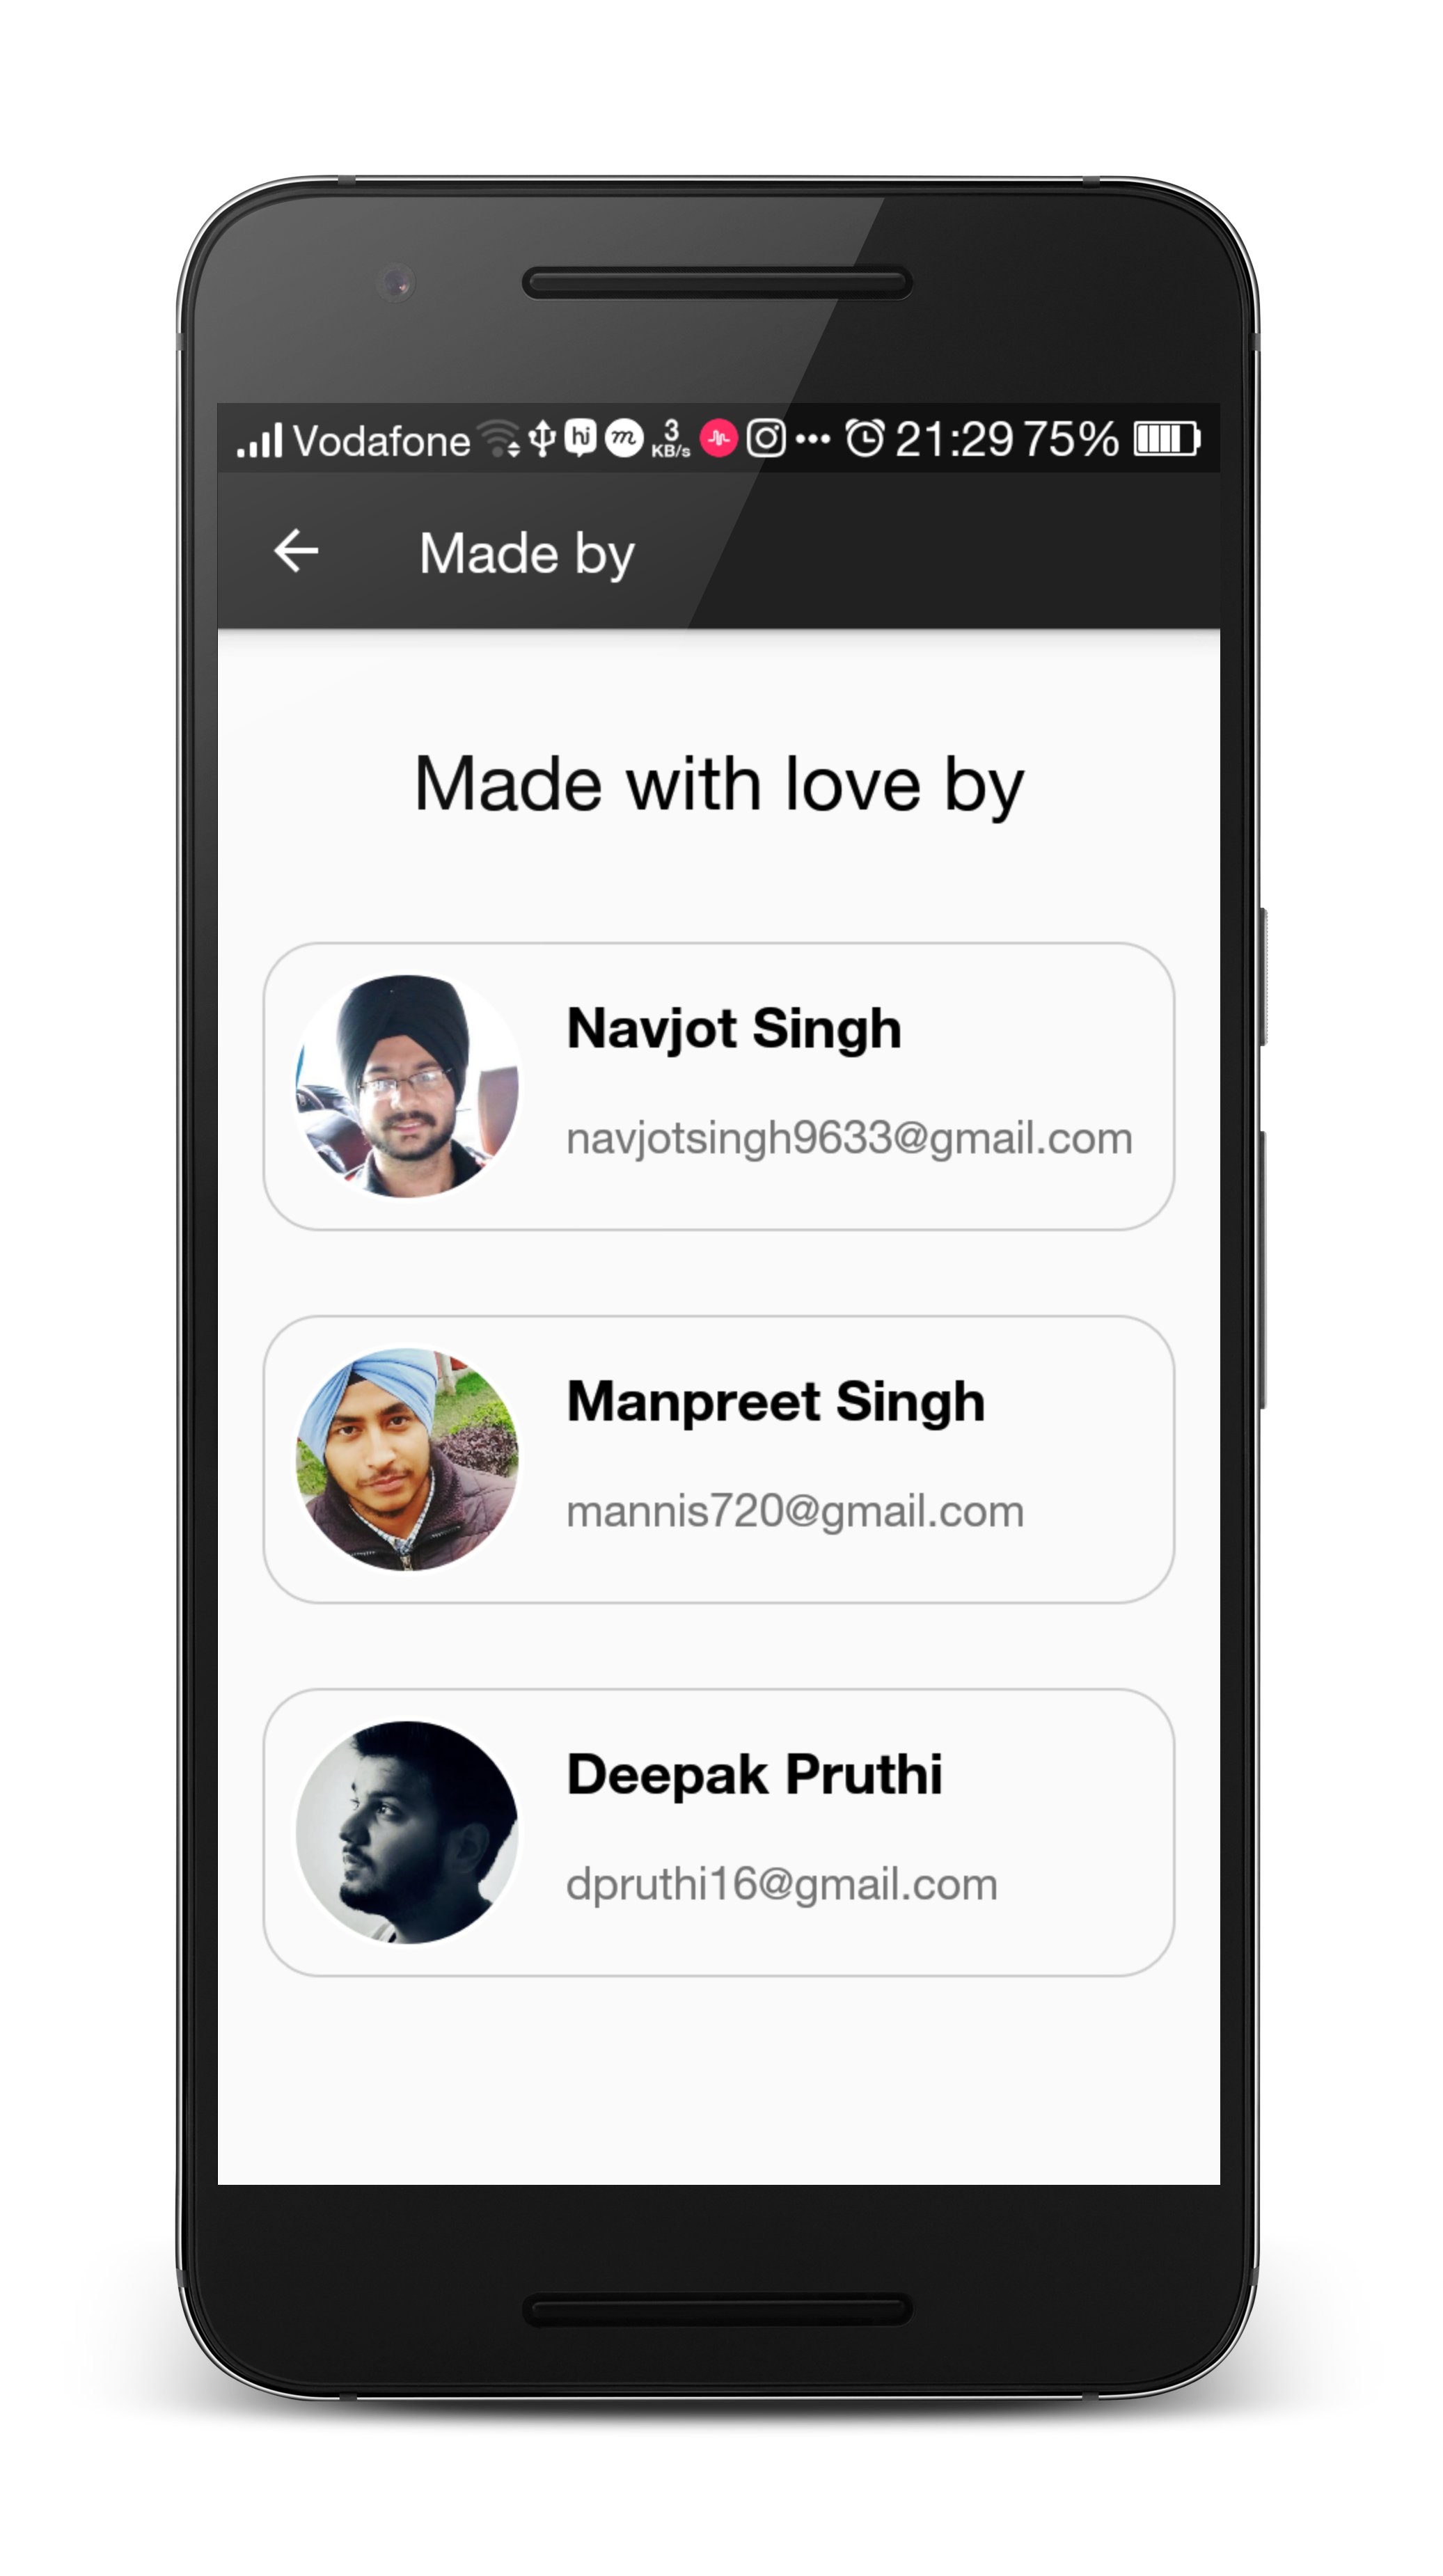
\includegraphics[scale=0.13]{images/d2.png}
\caption{Screen 17}
\end{figure}



\section{Back Ends Representation (Database to be used)}
\subsection{Snapshots of Database Tables with brief description}